\documentclass[12pt,a4paper]{article}

\usepackage[utf8]{inputenc}
\usepackage[T1]{fontenc}
\usepackage[italian]{babel}
\usepackage{graphicx}
\usepackage{longtable}
\usepackage{array}
\usepackage{geometry}
\usepackage[table]{xcolor}
\usepackage{fancyhdr}
\usepackage{titlesec}
\usepackage{hyperref}
\usepackage{float}
\usepackage{caption}
\usepackage{enumitem}

\geometry{margin=2.5cm}
\setlength{\parindent}{0pt}
\setlength{\parskip}{\baselineskip}
\captionsetup[table]{position=bottom}

\definecolor{lightblue}{RGB}{10,160,255}
\definecolor{unipablue}{RGB}{0,70,127}

\hypersetup{
    colorlinks=true,
    linkcolor=unipablue,
    urlcolor=unipablue,
    pdftitle={RAD},
    pdfauthor={Simone Sottile, Matteo Duca, Giuseppe Giacomarra, Gilberto Mogavero}
}

\pagestyle{fancy}
\setlength{\headheight}{14.5pt}
\fancyhf{}
\fancyhead[L]{\small\textit{AFAM Connect}}
\fancyhead[R]{\small\textit{RAD}}
\fancyfoot[C]{\thepage}
\renewcommand{\headrulewidth}{0.4pt}
\fancypagestyle{plain}{
    \fancyhf{}
    \fancyfoot[C]{\thepage}
    \renewcommand{\headrulewidth}{0pt}
}

\titleformat{\section}
  {\normalfont\Large\bfseries\color{unipablue}}
  {\thesection}{1em}{}[{\color{unipablue}\titlerule[0.5pt]}]

\titleformat{\subsection}
  {\normalfont\large\bfseries}
  {\thesubsection}{1em}{}

\titleformat{\paragraph}[block]
  {\normalfont\normalsize\bfseries}
  {\theparagraph}{1em}{}

\titleformat{\subparagraph}[block]
  {\normalfont\normalsize\bfseries}
  {\thesubparagraph}{1em}{}

\titlespacing*{\paragraph}{0pt}{1.25em}{0.5em}
\titlespacing*{\subparagraph}{0pt}{1em}{0.4em}

\setcounter{secnumdepth}{5}
\setcounter{tocdepth}{5}

\newcommand{\spaziocontenuto}{\mbox{}\par\vspace{1.2cm}}

\begin{document}

\pagenumbering{arabic}
\setcounter{page}{1}
\begin{minipage}[t][\dimexpr\textheight-1cm\relax][t]{\textwidth}
    \thispagestyle{plain}
    \centering

    
\includegraphics[width=0.25\textwidth]{logo-unipa.png}

    \vspace{0.5cm}
    {\large\textsc{Università degli Studi di Palermo}\par}
    \vspace{0.15cm}
    {\small\textsc{Dipartimento di Ingegneria --- A.A. 2025/2026}\par}

    \vspace{1.8cm}

    \resizebox{\textwidth}{!}{%
        \textbf{\color{unipablue}Requirements Analysis Document}%
    }

    \vspace{0.8cm}
    
\includegraphics[width=0.5\textwidth]{pdf/logoIDS.png}

    \vfill

    {\large\textbf{Gruppo di lavoro}\par}
    \vspace{0.4cm}
    {\large
        Simone Sottile\\
        Matteo Duca\\
        Giuseppe Giacomarra\\
        Gilberto Mogavero
    \par}

    \vspace{1.5cm}
\end{minipage}
\newpage

\tableofcontents
\newpage

\section{Introduzione}

\subsection{Obiettivo generale}
L’obiettivo del progetto è quello di realizzare una piattaforma software in grado di fornire supporto alle istituzioni AFAM (Alta Formazione Artistica, Musicale e Coreutica) e ai relativi studenti, agendo da intermediario sicuro e centralizzato tra l'artista, l'istituzione e i soggetti valutatori esterni. 

Il sistema mira a digitalizzare e valorizzare il percorso artistico dei candidati, fornendo uno strumento idoneo alla creazione di un portfolio multimediale certificato e modulabile sotto il profilo della privacy. 

Questo documento descrive il software in termini di requisiti funzionali e non funzionali, definendo in modo univoco le regole di dominio dell'applicazione (quali le politiche anti-download, i limiti di storage e la temporizzazione delle condivisioni). Esso funge da specifica tecnica formale e da base contrattuale tra il committente e gli sviluppatori della piattaforma.
\spaziocontenuto

\subsection{Definizioni, acronimi e abbreviazioni del Sistema}

\subsubsection{Definizioni}
\small
\begin{longtable}{|
>{\columncolor{unipablue}\color{white}\bfseries\raggedright\arraybackslash}p{3.4cm}|
>{\raggedright\arraybackslash}p{10.2cm}|}
\hline
\multicolumn{1}{|c|}{\cellcolor{unipablue}\color{white}\rule{0pt}{2.7ex}\textbf{TERMINE}} &
\multicolumn{1}{c|}{\rule{0pt}{2.7ex}\textbf{SIGNIFICATO}} \\
\hline
Studente & Utilizzatore autenticato del Sistema, appartenente a un'istituzione AFAM, che gestisce il proprio profilo e portfolio artistico. \\ \hline
Utente Esterno & Soggetto terzo non registrato (es. membro di commissione, ente valutatore) che consulta i materiali autorizzati dallo studente. \\ \hline
Credenziali locali & Insieme di dati personali necessari allo studente per autenticarsi direttamente sulla piattaforma, composti da e-mail e password. \\ \hline
Identità Digitale & Sistema di autenticazione federata nazionale ed europea (\textbf{SPID} e \textbf{eIDAS}) che permette la verifica e l'accesso sicuro dell'utente tramite Identity Provider esterni. \\ \hline
Portfolio Artistico & Raccolta digitalizzata e centralizzata della produzione d'ingegno dello studente, comprendente asset multimediali, spartiti e curriculum. \\ \hline
Categoria Artistica & Raggruppamento logico e categoriale (es. Pianoforte, Danza) creato dallo studente per organizzare i propri file nel sistema. \\ \hline
Contenuto Pubblico & Stato di privacy di un file che lo rende visibile a chiunque effettui una ricerca standard sulla piattaforma o acceda tramite link esterno. \\ \hline
Contenuto Privato & Stato di privacy di un file che lo rende invisibile alla ricerca standard, sbloccabile esclusivamente tramite inserimento di un codice univoco. \\ \hline
Link di Condivisione & URL univoco e temporizzato generato dallo studente per consentire ai valutatori esterni l'accesso sincrono e asincrono ai soli file pubblici selezionati. \\ \hline
Codice di Sblocco & Token testuale generato dallo studente per abilitare la consultazione protetta di contenuti privati a specifici destinatari interni all'istituzione. \\ \hline
Ricevuta di Lettura & Indicatore visivo automatizzato che notifica allo studente l'avvenuta apertura e consultazione di un link inviato all'esterno. \\ \hline
Streaming controllato & Modalità di fruizione inline dei flussi audio/video e dei documenti PDF che inibisce nativamente qualsiasi operazione di download del file fisico. \\ \hline
\caption{Glossario e Definizioni dei termini del dominio AFAM}
\label{tab:definizioni_sistema}\\
\end{longtable}
\normalsize

\subsubsection{Acronimi e Abbreviazioni}
\begin{table}[H]
\centering
\small
\begin{tabular}{|
>{\columncolor{unipablue}\color{white}\bfseries\raggedright\arraybackslash}p{3.4cm}|
>{\raggedright\arraybackslash}p{10.2cm}|}
\hline
\multicolumn{1}{|c|}{\cellcolor{unipablue}\color{white}\rule{0pt}{2.7ex}\textbf{ACRONIMO}} &
\multicolumn{1}{c|}{\rule{0pt}{2.7ex}\textbf{SIGNIFICATO}} \\
\hline
AFAM & Alta Formazione Artistica, Musicale e Coreutica. \\ \hline
DBMS & Database Management System (Sistema per la gestione di basi di dati). \\ \hline
SPID & Sistema Pubblico di Identità Digitale. \\ \hline
eIDAS & electronic IDentification Authentication and Signature. \\ \hline
AgID & Agenzia per l'Italia Digitale. \\ \hline
OTP / 2FA & One-Time Password / Autenticazione a Due Fattori. \\ \hline
GUI & Graphical User Interface (Interfaccia Grafica Utente). \\ \hline
URL & Uniform Resource Locator (Link/Indirizzo Web). \\ \hline
\end{tabular}
\caption{Acronimi e Abbreviazioni tecniche utilizzate nel documento}
\label{tab:acronimi_sistema}
\end{table}

\section{Sistema attuale}
Supponiamo che non esista alcun sistema informatizzato preesistente in uso dagli istituti.
\spaziocontenuto

\section{Sistema proposto}

\subsection{Vista d’insieme}
La proposta progettuale prevede un software in grado di supportare gli studenti delle istituzioni AFAM nella gestione e valorizzazione della propria identità digitale e della produzione artistica, automatizzando e semplificando attività quali l'organizzazione del portfolio multimediale, la regolazione della privacy dei contenuti e la gestione delle condivisioni sia interne che esterne.

La strutturazione dei contenuti in categorie artistiche personalizzate permette allo studente di stabilire con certezza il livello di visibilità di ogni singola opera, tenendo traccia dei file caricati e modificando la privacy tra Pubblico o Privato. In questo modo, anche la consultazione da parte di terzi risulta controllata e permette di determinare molto più facilmente quali materiali mostrare in base allo specifico contesto (es. audizioni, esami o concorsi).

Questo tipo di software consente inoltre di mantenere centralizzate le informazioni sul percorso dello studente, rendendo più semplice e veloce la condivisione mirata di queste informazioni senza dover ricorrere all'invio frammentato di email, e fornendo una panoramica completa e protetta della produzione d'ingegno del candidato. 

Il software prevede inoltre funzioni di tracciamento e feedback al fine di aiutare gli studenti ad avere un riscontro oggettivo sulle proprie candidature, mostrando notifiche visive immediate non appena i link inviati vengono effettivamente aperti e consultati.

Di seguito sono illustrate le interfacce che consentono di svolgere le funzionalità principali del software:
\begin{itemize}
    \item \textbf{Schermata di Login / Autenticazione:} Interfaccia che permette di effettuare l'accesso sicuro al sistema tramite credenziali locali standard (protette da codice OTP inviato via e-mail) o, in alternativa, tramite i sistemi di identità digitale \textbf{SPID} ed \textbf{eIDAS} previa selezione del proprio Provider dall'apposito menu a tendina. Include anche il form di registrazione e di recupero password.
    \item \textbf{Area Personale (Home AFAM / Dashboard Studente):} Interfaccia principale a cui accede lo studente una volta autenticato. Da qui l'utente può navigare verso la gestione del proprio profilo anagrafico e del background artistico, oppure accedere alla gestione dei contenuti e delle condivisioni.
    \item \textbf{Schermata Gestione Contenuti ed Elenco File:} Interfaccia che permette di visualizzare e creare le Categorie Artistiche e di effettuare l'upload dei file (audio, video, PDF) entro il limite di 1 GB. Tramite menu a tendina contestuali (attivati dal pulsante "+"), consente di modificare, eliminare o regolare lo stato di privacy (Pubblico/Privato) di ciascun asset.
    \item \textbf{Schermata Gestione Condivisione (Link e Codici):} Interfaccia sdoppiata che permette allo studente di selezionare i materiali e generare URL univoci temporizzati per l'esterno (della durata di 14 giorni con indicatore di avvenuta lettura) attingendo dai file pubblici, oppure codici di sblocco univoci per la condivisione interna di file privati, con relative funzioni di revoca manuale immediata.
    \item \textbf{Schermata di Ricerca e Consultazione Profilo:} Interfaccia dedicata agli utenti della piattaforma e ai valutatori esterni. Permette di cercare uno studente per nome e cognome per consultarne il profilo pubblico o, tramite l'inserimento di un codice valido o la risoluzione di un link di condivisione esterno, accedere ai file multimediali e documentali autorizzati.
    \item \textbf{Schermate di Fruizione (Player e Visualizzatore):} Interfacce integrate per la fruizione protetta dei contenuti che si adattano al formato del file selezionato (Riproduttore Multimediale per audio/video in streaming e Visualizzatore Documenti per i PDF), inibendo nativamente qualsiasi funzione di download.
\end{itemize}
\spaziocontenuto
\subsection{Requisiti funzionali}
Il Sistema prevede due macro-tipologie di attori, nello specifico lo Studente e l'Utente (Generico/Esterno), le cui interazioni con la piattaforma sono governate dai flussi logici e dai macro casi d'uso descritti di seguito:

\subsubsection{Funzionalità per lo Studente (Macro Casi d'Uso)}
Il software centralizza la gestione della presenza digitale degli studenti AFAM, strutturando le interazioni principali nei seguenti macro casi d'uso:

\begin{itemize}
    \item \textbf{Autenticazione e Accesso Federato:} Permette l'accesso sicuro all'Area Personale dello studente. Il flusso prevede la verifica delle credenziali locali standard, protette da autenticazione a due fattori (2FA) tramite codice OTP monouso inviato via e-mail, oppure il reindirizzamento verso i gateway di identità digitale federata \textbf{SPID} ed \textbf{eIDAS}. Include le procedure di registrazione locale (previa validazione di un codice di attivazione), il recupero password self-service e la terminazione della sessione (logout).
    \item \textbf{Gestione Profilo e Background Artistico:} Consente allo studente di amministrare le informazioni relative alla propria identità accademica e artistica. L'attore può inserire, modificare o eliminare i propri dati anagrafici e le voci relative alle esperienze passate, quali istituti frequentati, collaborazioni stabili o partecipazioni a eventi e concorsi, aggiornando i record sul database (DBMS).
    \item \textbf{Gestione Portfolio e Categorie Artistiche:} Regola l'organizzazione e l'ingestion della produzione d'ingegno dello studente. Il flusso permette di creare e personalizzare Categorie Artistiche dedicate (es. Pianoforte, Canto) ed effettuare l'upload dei file multimediali o documentali (audio, video, PDF) inserendo un titolo e una descrizione per ciascun asset caricato.
    \item \textbf{Modulazione della Privacy dei Contenuti:} Abilita lo studente a variare in tempo reale le politiche di sicurezza e visibilità dei propri file sul database. L'utente può impostare lo stato di ogni singolo asset su \textit{Pubblico}, rendendolo rintracciabile nel sistema e associabile ai link esterni, oppure su \textit{Privato}, segregandolo dalla ricerca globale e vincolandolo all'uso di codici.
    \item \textbf{Condivisione Esterna tramite Link Temporizzati:} Gestisce la generazione di canali di consultazione remota per soggetti terzi. Lo studente seleziona un sottoinsieme di file impostati come \textit{Pubblici} e genera un URL univoco testuale crittografico. Il sistema offre un pannello di monitoraggio per visualizzare la ricevuta di lettura (spunta) all'apertura del link e permette la revoca manuale anticipata del collegamento.
    \item \textbf{Condivisione Interna tramite Codice di Sblocco:} Consente la distribuzione controllata di materiale protetto all'interno dell'istituzione. Lo studente seleziona i file impostati come \textit{Privati} e genera un codice alfanumerico univoco da veicolare ai destinatari d'interesse. Il modulo include una schermata riepilogativa per monitorare i codici emessi e revocarne i permessi in qualsiasi momento.
\end{itemize}

\spaziocontenuto

\subsubsection{Funzionalità per l'Utente Esterno (Macro Casi d'Uso)}
Il sistema governa l'accesso ai contenuti da parte di utenti terzi o della piattaforma attraverso specifiche interazioni che non richiedono la registrazione di un profilo nominale:
\begin{itemize}
    \item \textbf{Ricerca Globale e Consultazione Pubblica:} Permette a qualunque utente di individuare uno studente iscritto inserendo il relativo nome e cognome all'interno del motore di ricerca. Il flusso restituisce la visualizzazione dell'Area Personale del candidato limitata esclusivamente ai file multimediali e alle categorie che l'autore ha contrassegnato con stato di privacy \textit{Pubblico}.
    \item \textbf{Risoluzione Link di Condivisione Esterna:} Gestisce l'accesso guidato alla piattaforma da parte dei valutatori. All'inserimento dell'URL univoco, il sistema ne verifica la validità temporale (entro la scadenza di 14 giorni), notifica l'avvenuta lettura allo studente e reindirizza l'utente esterno a una schermata dedicata contenente unicamente il portfolio di file pubblici selezionati per quella candidatura.
    \item \textbf{Sblocco Contenuti Privati tramite Codice:} Consente la visualizzazione di asset protetti all'interno di un profilo cercato. Qualora l'utente esterno inserisca nell'apposita maschera grafica un codice di sblocco valido e associato a quel profilo, il sistema interroga il DBMS e abilita temporaneamente la visualizzazione inline dei corrispondenti file privati.
    \item \textbf{Fruizione Protetta degli Asset (Anti-Download):} Regola l'interazione con i singoli file multimediali e documentali durante la consultazione. La selezione di un asset inizializza automaticamente il player multimediale integrato per i flussi audio/video in streaming controllato, oppure il visualizzatore dedicato per i documenti PDF, inibendo nativamente qualsiasi funzione di scaricamento locale del file fisico.
\end{itemize}

\spaziocontenuto

\subsection{Requisiti non funzionali}

\subsubsection{Requisiti del Prodotto}
\begin{itemize}
    \item \textbf{Usabilità:} Un utente finale (studente o valutatore esterno) privo di competenze informatiche avanzate deve essere in grado di utilizzare autonomamente tutte le funzioni del sistema (upload asset, modifica privacy, generazione link/codici) dopo un tempo di auto-addestramento non superiore a 15 minuti. Il tasso medio di errore operativo per gli utenti esperti non deve superare una singola occorrenza per ora di utilizzo.
    \item \textbf{Tempi di risposta:} Il tempo di caricamento ed elaborazione delle maschere grafiche (refresh dello schermo) deve assestarsi su una media inferiore a 1.5 secondi in condizioni di normale carico di rete.
    \item \textbf{Vincoli di Spazio:} Il backend applica un controllo algoritmico in fase di ingestion dei file, rifiutando a livello di memoria qualsiasi asset fisico che superi la quota rigida di 1 GB per singolo upload e restituendo un feedback immediato di errore a video.
    \item \textbf{Affidabilità e Disponibilità:} Il sistema deve garantire un indice di disponibilità continua pari al $99.9\%$ in modalità $24/7$. Nelle finestre temporali di picco accademico (sessioni di esame o audizioni), il tempo massimo di inattività (downtime) non deve superare i 5 minuti complessivi nell'arco dell'intero mese.
    \item \textbf{Robustezza:} In caso di guasto imprevisto o caduta di connessione con il DBMS relazionale, la probabilità di corruzione dei dati transazionali memorizzati deve essere pari a zero ($0\%$). Il tempo di riavvio automatico del sistema dopo un malfunzionamento deve essere inferiore a 30 secondi.
    \item \textbf{Sicurezza:} Il sistema memorizza le password nel database previa applicazione dell'algoritmo di hashing unidirezionale SHA-256. Le interfacce integrano moduli player che inibiscono i flussi di download diretto, veicolando i contenuti esclusivamente tramite riproduzione in streaming controllato inline.
\end{itemize}

\subsubsection{Requisiti Organizzativi}
\begin{itemize}
    \item \textbf{Requisiti di Sviluppo e Processo:} Il backend logico e i moduli applicativi del sistema devono essere interamente sviluppati e implementati in linguaggio Java.
    \item \textbf{Requisiti Operativi:} Il sistema gestisce lo stato della sessione memorizzando temporaneamente l'identificativo dell'utente loggato. Al momento del logout o dopo un timeout di inattività di 30 minuti, il sistema cancella tali record volatili ripristinando la visualizzazione anonima.
    \item \textbf{Requisiti di Controllo Temporale:} Un modulo interno di batch scheduling si esegue automaticamente ogni giorno alle ore 00:00, effettuando una query sul DBMS per disattivare tutti i link di condivisione esterna che hanno superato il vincolo temporale di 14 giorni.
\end{itemize}

\subsubsection{Requisiti Esterni}
\begin{itemize}
    \item \textbf{Requisiti Legislativi e di Regolamentazione:} Il sistema implementa le politiche per la tutela dei dati personali in conformità con le normative GDPR, separando i file \textit{Pubblici} (accessibili via ricerca globale) da quelli \textit{Privati} (consultabili esclusivamente previa immissione di un codice di sblocco valido).
    \item \textbf{Requisiti di Interoperabilità e Standard:} Il sottosistema di identificazione digitale adotta gli standard di federazione \textbf{SAML 2.0} e \textbf{OpenID Connect} per permettere lo scambio dei flussi di autenticazione con i provider \textbf{SPID} ed \textbf{eIDAS} in conformità con le direttive \textbf{AgID}.
    \item \textbf{Interoperabilità Extra-Istituzionale:} L'architettura del software supporta l'estensione dei protocolli di comunicazione per consentire lo scambio di dati e la consultazione delle identità digitali in modo federato con sistemi analoghi di altre istituzioni della rete AFAM.
\end{itemize}
\subsection{Modelli di Sistema}
Si premette che nei casi d’uso elencati di seguito, con il termine ``Schermata di Login / Autenticazione'' si fa riferimento alla schermata di accesso principale del software, in cui lo studente può immettere le proprie credenziali locali o selezionare l'autenticazione federata tramite i gateway \textbf{SPID} o \textbf{eIDAS}. Con il termine ``Area Personale'' (o Dashboard Studente) si identifica l'interfaccia principale riservata allo studente autenticato, da cui si diramano i moduli di gestione del profilo, del portfolio e delle condivisioni. 

Con il termine ``Schermata di Ricerca e Consultazione Profilo'' si fa riferimento all'interfaccia globale di localizzazione degli iscritti; tale funzionalità è accessibile sia dall'utente esterno per scopi di valutazione, sia dallo studente stesso per visionare la resa pubblica del proprio portfolio o per ricercare altri utenti all'interno della piattaforma AFAM. Con il termine ``Schermate di Fruizione'' si identificano invece i componenti integrati (Player multimediale e Visualizzatore PDF) dedicati alla riproduzione protetta (anti-download) degli asset documentali e multimediali. Queste schermate sono condivise da tutte le tipologie di attori, consentendo allo studente la verifica dei propri materiali o la consultazione delle opere altrui, e all'utente esterno la sottomissione controllata dei file autorizzati.

Inoltre, all'interno di ciascuna interfaccia grafica del sistema, è capillarmente presente un pulsante di ``Annulla'', ``Indietro'' o ``Esci''. Questa scelta progettuale garantisce che l'utilizzatore possa interrompere in qualsiasi momento l'operazione corrente (come il caricamento di un file o la generazione di un codice) e fare ritorno in sicurezza alla schermata immediatamente precedente, ripristinando lo stato di consistenza della navigazione.\spaziocontenuto

\subsubsection{Vista degli attori}

\begin{figure}[H]
    \centering
    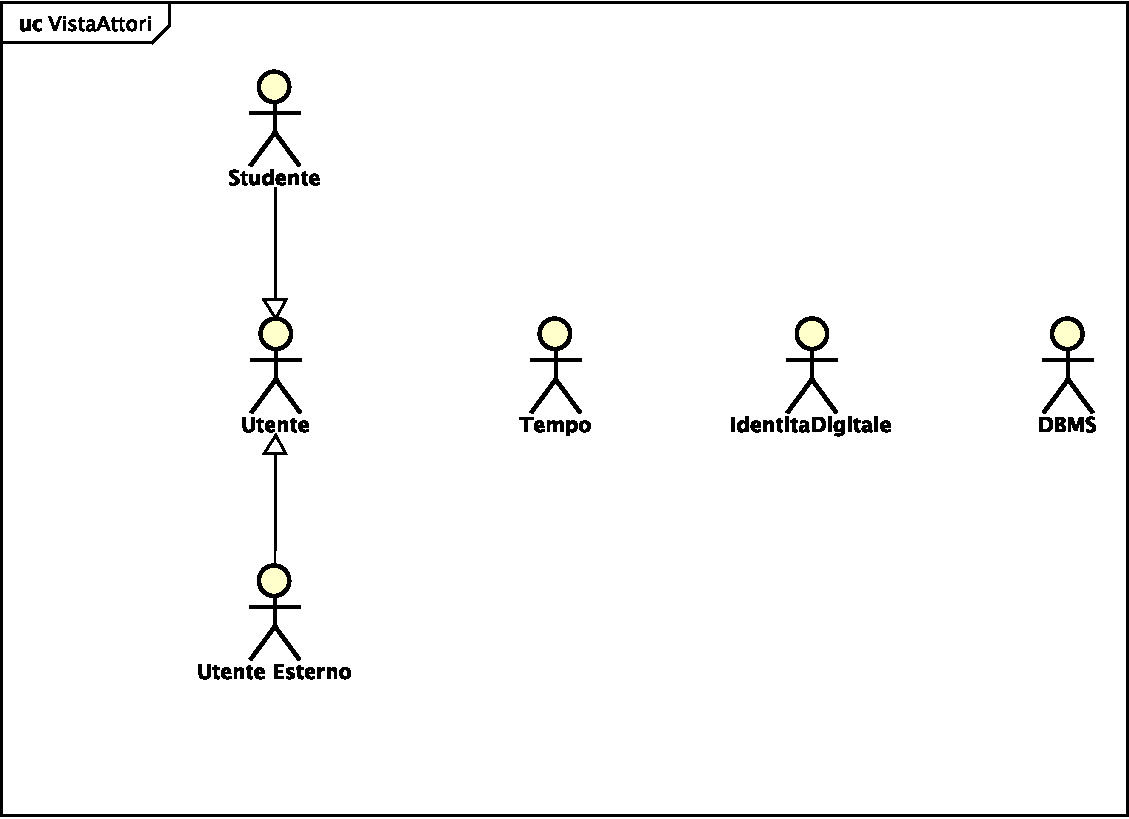
\includegraphics[width=\textwidth,height=0.70\textheight,keepaspectratio]{pdf/VistaAttori.pdf}
    \caption{Vista degli attori del sistema}
    \label{fig:vista_attori}
\end{figure}

All'interno del sistema sono stati individuati sei attori, suddivisi tra figure umane (utilizzatori della piattaforma) e componenti di sistema o temporali che innescano o supportano le procedure operative:

\small
\begin{longtable}{|
>{\columncolor{unipablue}\color{white}\bfseries\raggedright\arraybackslash}p{3.4cm}|
>{\raggedright\arraybackslash}p{10.2cm}|}
\hline
\multicolumn{1}{|c|}{\cellcolor{unipablue}\color{white}\rule{0pt}{2.7ex}\textbf{ATTORE}} &
\multicolumn{1}{c|}{\rule{0pt}{2.7ex}\textbf{DESCRIZIONE}} \\
\hline
Utente & Attore generico del sistema che rappresenta la classe base per chiunque interagisca con le funzioni pubbliche della piattaforma. Da esso ereditano sia lo Studente che l'Utente Esterno la facoltà di effettuare ricerche globali e fruire degli asset multimediali pubblici. \\ \hline
Studente & Attore autenticato utilizzatore del sistema, appartenente a un'istituzione AFAM. Possiede i massimi privilegi di scrittura e gestione sul proprio spazio, potendo modificare l'anagrafica, caricare file, modularne la privacy e generare o revocare link e codici di sblocco. \\ \hline
Utente Esterno & Attore non registrato (es. membro di commissione, docente esterno, ente partner) che interagisce con la piattaforma in modalità di sola lettura per consultare i percorsi e i file multimediali degli studenti, previo possesso di un URL valido o di un codice di sblocco. \\ \hline
Identità Digitale & Attore di sistema esterno che rappresenta il gateway di autenticazione federata nazionale ed europea (\textbf{SPID} ed \textbf{eIDAS}). Fornisce alla piattaforma i payload e i token di identità necessari a validare in sicurezza l'accesso o l'iscrizione degli studenti. \\ \hline
DBMS & Attore di sistema che si occupa della persistenza e dell'immagazzinamento sicuro di tutti i dati applicativi, tra cui i record anagrafici, i percorsi fisici dei file multimediali, lo stato di privacy degli asset e i token dei link di condivisione. \\ \hline
Tempo & Attore di sistema non umano che incorpora lo scorrere del tempo come evento scatenante (trigger). Agisce in modo automatizzato per avviare le procedure batch periodiche, come il controllo quotidiano e la conseguente disattivazione dei link scaduti. \\ \hline
\caption{Mappatura e descrizione degli Attori del sistema AFAM}
\label{tab:descrizione_attori}\\
\end{longtable}
\normalsize

\newpage
\subsubsection{Modelli dei casi d'uso}

\paragraph{Vista d'insieme}
La seguente immagine mostra la vista d’insieme del sistema proposto.

\begin{figure}[H]
    \centering
    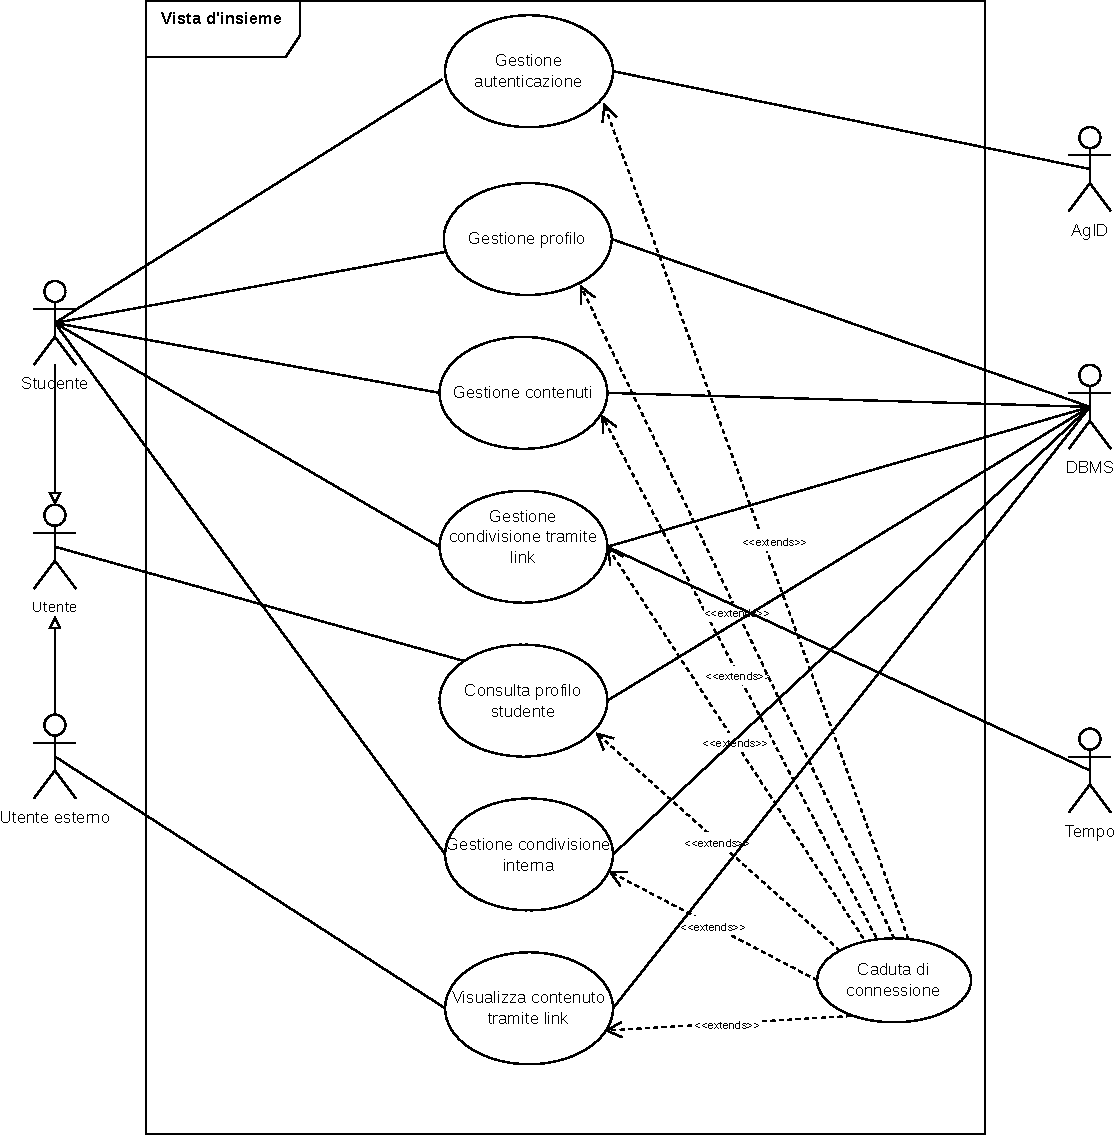
\includegraphics[width=\textwidth,height=0.82\textheight,keepaspectratio]{pdf/Vistad'insieme-crop.pdf}
    \caption{Vista d'insieme del sistema}
    \label{fig:vista_dinsieme}
\end{figure}


\newpage

Le funzionalità principali del sistema vengono riassunte e formalizzate nella seguente tabella orientata alla descrizione dei macro casi d'uso:
\spaziocontenuto

\small
\begin{longtable}{|
>{\columncolor{unipablue}\color{white}\bfseries\raggedright\arraybackslash}p{4.1cm}|
>{\raggedright\arraybackslash}p{9.5cm}|}
\hline
Gestione autenticazione & Gestisce tutte le procedure relative all'accesso al sistema. Permette allo studente di registrarsi alla piattaforma creando un nuovo account e di effettuare l'accesso alla propria area personale. L'autenticazione può avvenire tramite credenziali standard (email e password) oppure tramite i servizi di identità digitale (SPID o eIDAS). Infine, sono previste le funzionalità per il recupero della password e per la disconnessione sicura dal sistema. \\ \hline
Gestione profilo & Gestisce le funzionalità di consultazione e aggiornamento delle informazioni personali e curriculari dell'utente. Nello specifico, permette allo studente di inserire e modificare i propri dati personali e di arricchire il proprio profilo aggiungendo o aggiornando il proprio background artistico (percorso di studi, collaborazioni ed esperienze pregresse). \\ \hline
Gestione contenuti & Permette allo studente di gestire integralmente la propria area artistica: dalla creazione di specifiche categorie di interesse, all'upload di nuovi file (suddivisi per strumenti, tracce audio, file video, immagini, pdf). Inoltre, permette la modifica o l'eliminazione dei materiali precedentemente caricati e la configurazione della privacy per ogni singolo contenuto. \\ \hline
Gestione condivisione tramite link & Permette allo studente di selezionare specifici contenuti, precedentemente caricati, e di generare link per la diffusione del materiale a utenti o commissioni esterne all'istituzione AFAM. Inoltre, permette una gestione completa delle condivisioni attive, consentendo allo studente di visualizzare l'elenco dei link generati, monitorarne la data e l'ora di scadenza automatica e la possibilità di revocare il link prima del termine previsto. \\ \hline
Consulta profilo studente & Permette la ricerca e la consultazione dei profili degli studenti registrati alla piattaforma AFAM. Consente all'utente (Studente o utente esterno) di cercare uno specifico profilo. L'accesso ai materiali è regolato in modo differenziato: è consentita la libera visualizzazione dei contenuti pubblici, mentre la visualizzazione dei contenuti privati avviene nell'apposita sezione a seguito dell'inserimento di un codice. \\ \hline
Gestione condivisione interna & Permette allo studente di condividere specifici contenuti privati con altri utenti, senza la necessità di generare un link. La condivisione avviene tramite la generazione di un codice univoco: l'utente destinatario, inserendo tale codice nell'apposita area, otterrà l'accesso alla visualizzazione dei contenuti privati selezionati dallo studente. Questa modalità non prevede alcuna verifica di riscontro della visualizzazione. È prevista inoltre la funzionalità che permette allo studente di monitorare lo storico dei codici creati e di revocarne la validità in qualsiasi momento. \\ \hline
Visualizza contenuto tramite link & Gestisce l'accesso da parte di soggetti terzi non registrati alla piattaforma. Consente all'utente esterno di accedere a un'area dedicata per visualizzare esclusivamente i contenuti multimediali selezionati e condivisi da uno studente AFAM. Il modulo garantisce un accesso tracciato aggiornando lo stato di visualizzazione per fornire il feedback allo studente. \\ \hline
\caption{Mappatura e descrizione dei Macro Casi d'Uso}
\label{tab:macro_casi_uso}\\
\end{longtable}
\normalsize

\spaziocontenuto
\newpage
\paragraph{Caso d'uso: Caduta di connessione}
Il seguente caso d'uso descrive la gestione delle anomalie di rete o di sistema in tutte quelle funzionalità che richiedono un'interazione transazionale con la base di dati, integrando un meccanismo di ripristino e sottomissione della richiesta.

\small
\begin{longtable}{|
>{\columncolor{unipablue}\color{white}\bfseries\raggedright\arraybackslash}p{3.4cm}|
>{\raggedright\arraybackslash}p{10.2cm}|}
\hline
\textbf{Caso d’uso} & Errore comunicazione DBMS \\ \hline
\textbf{ID} & 0.1 \\ \hline
\textbf{Attori} & Utente (iniziatore), DBMS (partecipante) \\ \hline
\textbf{Precondizioni} & Il sistema rileva l'impossibilità di stabilire o mantenere una connessione attiva con il database, oppure riceve un codice d'errore fatale durante una query. \\ \hline
\textbf{Flusso degli eventi} &
\begin{enumerate}
    \item L'Utente esegue un'operazione che richiede l'accesso in lettura o scrittura sul DBMS.
    \item Il Sistema intercetta il timeout o la mancata risposta del server della base di dati.
    \item Il Sistema mostra a video un messaggio di errore: ``Errore di comunicazione con il database'' e mette a disposizione i pulsanti ``Riprova'' e ``Annulla''.
    \item L'Utente seleziona il pulsante ``Annulla''.
    \item Il Sistema mostra a video la ``Schermata Principale''.
\end{enumerate} \\ \hline
\textbf{Flussi Alternativi} &
\textbf{2a. Tentativo di riconnessione (Riprova):}
\begin{itemize}
    \item[1.] Al punto 4 del flusso principale, l'Utente seleziona il pulsante ``Riprova''.
    \item[2.] Il Sistema effettua un nuovo tentativo di esecuzione della query sul DBMS.
    \item[3.] Se il tentativo ha esito positivo, la finestra di errore si chiude e il sistema riprende il normale flusso del caso d'uso originario dal quale era stato interrotto.
    \item[4.] Se il tentativo fallisce nuovamente, il sistema ritorna al punto 3 del flusso principale.
\end{itemize} \\ \hline
\textbf{Postcondizioni} & Il Sistema ha mostrato a video la ``Schermata Principale''. \\ \hline
\caption{Caso d'Uso : Caduta di connessione}
\label{tab:uc_errore_dbms}\\
\end{longtable}
\normalsize

\newpage

\paragraph{Caso d'uso : Gestione Autenticazione}
All'interno della suddetta macro-categoria sono presenti i seguenti casi d'uso di dettaglio:
\begin{itemize}
    \item \textbf{Login (1.1):}
    \item \textbf{Login tramite SPID/eIDAS(1.2):}
    \item \textbf{Registrazione (1.3):}
    \item \textbf{Recupera Password (1.4):} 
    \item \textbf{Logout (1.5):}
\end{itemize}

\begin{figure}[H]
    \centering
    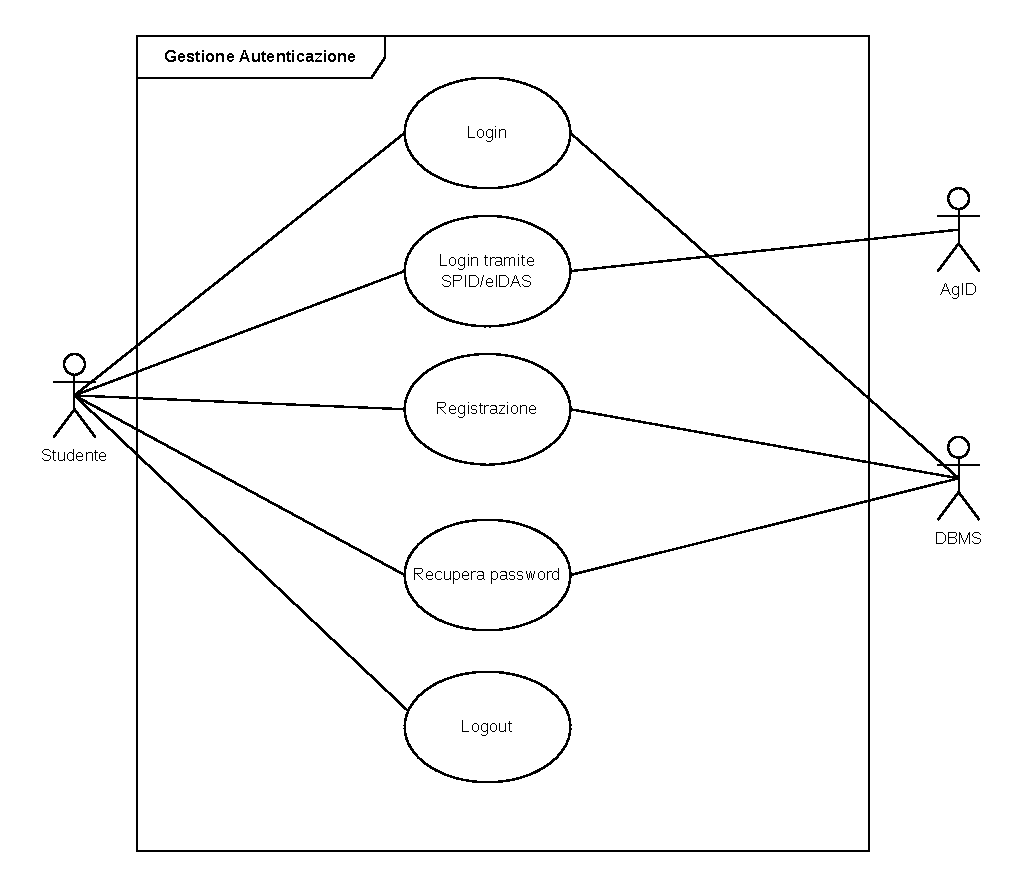
\includegraphics[width=\textwidth,height=1.2\textheight,keepaspectratio]{pdf/GestioneAutenticazione/GestioneAutenticazione.pdf}
    \caption{Vista d'insieme di Gestione Autenticazione}
    \label{fig:gestione_aut}
\end{figure}

\newpage

\subparagraph{Login}

Questo caso d'uso descrive la procedura di autenticazione a due fattori (2FA) eseguita dallo studente per accedere alla propria area riservata all'interno della piattaforma.

\small
\begin{longtable}{|
>{\columncolor{unipablue}\color{white}\bfseries\raggedright\arraybackslash}p{3.4cm}|
>{\raggedright\arraybackslash}p{10.2cm}|}
\hline
\textbf{Caso d’uso} & Login \\ \hline
\textbf{ID} & 1.1 \\ \hline
\textbf{Attori} & Studente (iniziatore), DBMS (partecipante) \\ \hline
\textbf{Precondizioni} & Il sistema ha mostrato a schermo la schermata principale. \\ \hline
\textbf{Flusso degli eventi} &
\begin{enumerate}
    \item Lo studente clicca sul pulsante ``Login''.
    \item Il Sistema mostra a video la schermata di login contenente il form (Email, Password) e il pulsante ``Accedi''.
    \item Lo studente compila i campi con Email e Password e clicca sul pulsante ``Accedi''.
    \item Il Sistema interroga il DBMS per verificare la presenza e la correttezza dei dati inseriti.
    \item \textbf{SE} le credenziali non sono corrette:
    \begin{itemize}
        \item[5.1.] Il Sistema mostra a video il messaggio di errore: ``Credenziali non corrette''.
        \item[5.2.] Lo studente clicca sul pulsante ``ok'' per chiuderlo.
        \item[5.3.] Il Sistema mostra nuovamente la schermata di login.
    \end{itemize}
\end{enumerate} \\
&
\begin{enumerate}
    \setcounter{enumi}{5}
    \item \textbf{ALTRIMENTI} (Credenziali corrette - Inizio verifica 2FA):
    \begin{itemize}
        \item[6.1.] Il Sistema genera un codice di verifica e lo invia all’e-mail dello studente.
        \item[6.2.] Il Sistema mostra a video la schermata ``Verifica Identità'' (campo Codice).
        \item[6.3.] Lo studente inserisce il codice ricevuto e clicca sul pulsante ``Verifica''.
        \item[6.4.] Il Sistema valida il codice inserito.
\end{itemize}
\end{enumerate} \\
&
\begin{itemize}
        \item[6.5.] \textbf{SE} il codice di verifica è errato:
        \begin{itemize}
            \item[6.5.1.] Il Sistema mostra a video il messaggio di errore: ``Codice errato''.
            \item[6.5.2.] Lo studente clicca sul pulsante ``Invia nuovo codice''.
            \item[6.5.3.] Il Sistema genera un nuovo codice, lo invia all’e-mail dello studente e ricarica la schermata di verifica.
        \end{itemize}
        \item[6.6.] \textbf{ALTRIMENTI} (il codice di verifica è corretto):
        \begin{itemize}
            \item[6.6.1.] Il Sistema richiede al DBMS i dati relativi all’Account.
            \item[6.6.2.] Il Sistema mostra a video la schermata ``Home AFAM''.
        \end{itemize}
\end{itemize} \\ \hline
\textbf{Postcondizioni} &
\begin{enumerate}
    \item Il Sistema ha mostrato la schermata ``Home AFAM''.
    \item Il Sistema ha mostrato a video la schermata di login.
\end{enumerate} \\ \hline
\textbf{Requisiti speciali} &
\begin{itemize}
    \item L'e-mail deve contenere una ``@'' e almeno un ``.''.
    \item La password deve contenere da un minimo di 8 a un massimo di 16 caratteri.
\end{itemize} \\ \hline
\caption{Scheda di dettaglio del Caso d'Uso Login}
\label{tab:uc_login}\\
\end{longtable}
\normalsize

\newpage
\subparagraph{Login tramite SPID/eIDAS}

Questo caso d'uso descrive la procedura di autenticazione federata eseguita dallo studente tramite un Provider SPID o eIDAS.

\small
\begin{longtable}{|
>{\columncolor{unipablue}\color{white}\bfseries\raggedright\arraybackslash}p{3.4cm}|
>{\raggedright\arraybackslash}p{10.2cm}|}
\hline
Caso d’uso & Login tramite SPID/eIDAS \\ \hline
ID & 1.2 \\ \hline
Attori & Studente (iniziatore), AgID e DBMS (partecipanti) \\ \hline
Precondizioni & Il Sistema ha mostrato a schermo la schermata principale. \\ \hline
Flusso degli eventi &
\begin{enumerate}
    \item Lo studente clicca sul pulsante ``Login''.
    \item Il Sistema mostra a video la schermata di login contenente il pulsante ``Entra con SPID/eIDAS''.
    \item Lo studente clicca sul pulsante ``Entra con SPID/eIDAS''.
    \item Il Sistema mostra a video un menu a tendina contenente l'elenco dei Provider disponibili.
    \item Lo studente seleziona il proprio Provider cliccando sull'apposita voce del menu.
\end{enumerate} \\
&
\begin{enumerate}
    \setcounter{enumi}{5}
    \item Il Sistema mostra a schermo il form di autenticazione del Provider scelto.
    \item Lo studente inserisce le proprie credenziali nel form e clicca sul pulsante ``Conferma''.
    \item Il Sistema richiede al Provider l'esito dell'autenticazione.
    \item Il Provider invia al Sistema l'esito e il codice fiscale associato all'autenticazione.
    \item \textbf{SE} l'esito è negativo:
    \begin{itemize}
        \item[10.1.] Il Sistema mostra a video il messaggio di errore: ``Accesso negato: clicca qui per registrarti''.
        \item[10.2.] Lo studente clicca sul pulsante ``Registrati'' per chiudere il messaggio di errore.
        \item[10.3.] Il Sistema invoca il caso d'uso ``Registrazione Studente''.
    \end{itemize}
\end{enumerate} \\
&
\begin{enumerate}
    \setcounter{enumi}{10}
    \item \textbf{ALTRIMENTI} (esito positivo):
    \begin{itemize}
        \item[11.1.] Il Sistema interroga il DBMS per verificare se lo studente è registrato alla piattaforma.
        \item[11.2.] \textbf{SE} lo studente non è registrato:
        \begin{itemize}
            \item[11.2.1.] Il Sistema mostra a video il messaggio di errore: ``Accesso negato: clicca qui per registrarti''.
            \item[11.2.2.] Lo studente clicca sul pulsante ``Registrati'' per chiudere il messaggio di errore.
            \item[11.2.3.] Il Sistema invoca il caso d'uso ``Registrazione Studente''.
        \end{itemize}
        \item[11.3.] \textbf{ALTRIMENTI}:
        \begin{itemize}
            \item[11.3.1.] Il Sistema richiede al DBMS i dati relativi all'account.
            \item[11.3.2.] Il Sistema mostra a video la schermata ``Home AFAM''.
        \end{itemize}
    \end{itemize}
\end{enumerate} \\ \hline
Postcondizioni &
\begin{enumerate}
    \item Il Sistema ha mostrato la schermata ``Home AFAM''.
    \item Il Sistema ha mostrato a video la schermata di login.
\end{enumerate} \\ \hline
\caption{Scheda di dettaglio del Caso d'Uso Login tramite SPID/eIDAS}
\label{tab:uc_login_spid_eidas}\\
\end{longtable}
\normalsize

\newpage
\subparagraph{Registrazione}

Questo caso d'uso descrive la procedura con cui lo studente crea e attiva un nuovo account sulla piattaforma.

\small
\begin{longtable}{|
>{\columncolor{unipablue}\color{white}\bfseries\raggedright\arraybackslash}p{3.4cm}|
>{\raggedright\arraybackslash}p{10.2cm}|}
\hline
Caso d’uso & Registrazione \\ \hline
ID & 1.3 \\ \hline
Attori & Studente (iniziatore), DBMS (partecipante) \\ \hline
Precondizioni & Il Sistema ha mostrato a schermo la schermata principale. \\ \hline
Flusso degli eventi &
\begin{enumerate}
    \item Lo studente clicca sul pulsante ``Registrati''.
    \item Il Sistema mostra a video la schermata ``Registrazione'' contenente:
    \begin{itemize}
        \item il form con i campi Nome, Cognome, Codice fiscale, E-mail, Password e Conferma Password;
        \item i pulsanti ``Conferma'' e ``Annulla''.
    \end{itemize}
    \item Lo studente compila i campi del form e clicca sul pulsante ``Conferma''.
    \item Il Sistema valida la corrispondenza delle password e il formato dei dati.
    \item \textbf{SE} i dati non sono validi o le password non corrispondono:
    \begin{itemize}
        \item[5.1.] Il Sistema mostra a video il messaggio di errore: ``Dati non validi''.
        \item[5.2.] Lo studente clicca sul pulsante ``ok'' per chiuderlo.
        \item[5.3.] Il Sistema mostra nuovamente la schermata ``Registrazione''.
    \end{itemize}
    \item \textbf{ALTRIMENTI} (dati validi):
    \begin{itemize}
        \item[6.1.] Il Sistema interroga il DBMS per verificare se l'e-mail è già presente.
    \end{itemize}
\end{enumerate} \\
&
\begin{enumerate}
    \setcounter{enumi}{6}
    \item \textbf{SE} l'e-mail è già registrata:
    \begin{itemize}
        \item[7.1.] Il Sistema mostra a video il messaggio di errore: ``E-mail già in uso''.
        \item[7.2.] Lo studente clicca sul pulsante ``ok'' per chiuderlo.
        \item[7.3.] Il Sistema mostra nuovamente la schermata ``Registrazione''.
    \end{itemize}
\end{enumerate} \\
&
\begin{enumerate}
    \setcounter{enumi}{7}
    \item \textbf{ALTRIMENTI} (e-mail non presente):
    \begin{itemize}
        \item[8.1.] Il Sistema genera un codice di attivazione e lo invia all'e-mail dello studente.
        \item[8.2.] Il Sistema mostra a video la schermata ``Attivazione Account'' contenente il campo ``Codice di attivazione''.
    \end{itemize}
    \item Lo studente inserisce il codice ricevuto e clicca sul pulsante ``Verifica''.
    \item Il Sistema verifica la validità del codice inserito.
    \item \textbf{SE} il codice è errato:
    \begin{itemize}
        \item[11.1.] Il Sistema mostra a video il messaggio di errore: ``Codice non valido''.
        \item[11.2.] Lo studente clicca sul pulsante ``Invia nuovo codice''.
        \item[11.3.] Il Sistema genera un nuovo codice, lo invia all'e-mail e ricarica la schermata di attivazione.
    \end{itemize}
\end{enumerate} \\
&
\begin{enumerate}
    \setcounter{enumi}{11}
    \item \textbf{ALTRIMENTI} (codice corretto):
    \begin{itemize}
        \item[12.1.] Il Sistema invia i dati del nuovo Studente al DBMS per la memorizzazione definitiva.
        \item[12.2.] Il Sistema mostra a video il messaggio di conferma: ``Registrazione completata''.
        \item[12.3.] Lo studente clicca sul pulsante ``ok'' per chiuderlo.
        \item[12.4.] Il Sistema mostra a video la schermata di ``Login''.
    \end{itemize}
\end{enumerate} \\ \hline
Postcondizioni &
\begin{enumerate}
    \item Il Sistema ha mostrato a video la schermata di login.
    \item Il Sistema ha mostrato a video la schermata per la registrazione.
\end{enumerate} \\ \hline
Requisiti speciali &
\begin{itemize}
    \item Il nome deve essere diverso dal cognome.
    \item Il nome deve contenere solo caratteri alfabetici.
    \item Il cognome deve contenere solo caratteri alfabetici.
    \item Il codice fiscale deve contenere 16 caratteri.
    \item L'e-mail deve contenere una ``@'' e almeno un ``.''.
    \item La password deve contenere da un minimo di 8 a un massimo di 16 caratteri, almeno una lettera maiuscola e almeno un numero.
\end{itemize} \\ \hline
\caption{Scheda di dettaglio del Caso d'Uso Registrazione}
\label{tab:uc_registrazione}\\
\end{longtable}
\normalsize

\newpage
\subparagraph{Recupera password}

Questo caso d'uso descrive la procedura con cui lo studente recupera l'accesso al proprio account impostando una nuova password.

\small
\begin{longtable}{|
>{\columncolor{unipablue}\color{white}\bfseries\raggedright\arraybackslash}p{3.4cm}|
>{\raggedright\arraybackslash}p{10.2cm}|}
\hline
Caso d’uso & Recupera password \\ \hline
ID & 1.4 \\ \hline
Attori & Studente (iniziatore), DBMS (partecipante) \\ \hline
Precondizioni & Il Sistema ha mostrato a schermo la schermata principale. \\ \hline
Flusso degli eventi &
\begin{enumerate}
    \item Lo studente clicca sul pulsante ``Recupera password''.
    \item Il Sistema mostra il form per il recupero della password.
    \item Lo studente inserisce la propria e-mail.
    \item Lo studente clicca sul pulsante ``Conferma''.
    \item Il Sistema verifica presso il DBMS se l'e-mail è associata a uno studente registrato.
    \item \textbf{SE} l'e-mail non esiste:
    \begin{itemize}
        \item[6.1.] Il Sistema mostra il messaggio di errore ``Studente non trovato''.
        \item[6.2.] Lo studente conferma la presa visione del messaggio.
        \item[6.3.] Il Sistema mostra nuovamente il form per il recupero della password.
    \end{itemize}
    \item \textbf{ALTRIMENTI} (l'e-mail esiste):
    \begin{itemize}
        \item[7.1.] Il Sistema genera un codice di recupero.
        \item[7.2.] Il Sistema invia all'e-mail dello studente il codice di recupero.
        \item[7.3.] Il Sistema mostra la schermata per l'inserimento del codice.
    \end{itemize}
\end{enumerate} \\
&
\begin{enumerate}
    \setcounter{enumi}{7}
    \item Lo studente inserisce il codice ricevuto.
    \item Lo studente clicca sul pulsante ``Conferma''.
    \item Il Sistema valida il codice inserito.
    \item \textbf{SE} il codice è errato:
    \begin{itemize}
        \item[11.1.] Il Sistema mostra il messaggio di errore ``Codice non valido''.
        \item[11.2.] Lo studente conferma la presa visione del messaggio.
        \item[11.3.] Il Sistema mostra nuovamente la schermata per l'inserimento del codice.
    \end{itemize}
\end{enumerate} \\
&
\begin{enumerate}
    \setcounter{enumi}{11}
    \item \textbf{ALTRIMENTI} (il codice è corretto):
    \begin{itemize}
        \item[12.1.] Il Sistema mostra il form per l'inserimento della nuova password.
        \item[12.2.] Lo studente inserisce la nuova password.
        \item[12.3.] Lo studente clicca sul pulsante ``Conferma''.
        \item[12.4.] Il Sistema aggiorna nel DBMS la password dello studente.
        \item[12.5.] Il Sistema mostra la schermata di login.
    \end{itemize}
\end{enumerate} \\ \hline
Postcondizioni &
\begin{enumerate}
    \item Il Sistema ha mostrato la schermata di login.
    \item Il Sistema ha mostrato il form per il recupero della password.
\end{enumerate} \\ \hline
Requisiti speciali &
\begin{itemize}
    \item L'e-mail deve contenere una ``@'' e almeno un ``.''.
    \item La password deve contenere da un minimo di 8 a un massimo di 16 caratteri, almeno una lettera maiuscola e almeno un numero.
\end{itemize} \\ \hline
\caption{Scheda di dettaglio del Caso d'Uso Recupera password}
\label{tab:uc_recupera_password}\\
\end{longtable}
\normalsize

\newpage
\subparagraph{Logout}

Questo caso d'uso descrive la procedura con cui lo studente termina la sessione attiva e si disconnette dalla piattaforma.

\small
\begin{longtable}{|
>{\columncolor{unipablue}\color{white}\bfseries\raggedright\arraybackslash}p{3.4cm}|
>{\raggedright\arraybackslash}p{10.2cm}|}
\hline
Caso d’uso & Logout \\ \hline
ID & 1.5 \\ \hline
Attori & Studente (iniziatore) \\ \hline
Precondizioni & Il Sistema ha mostrato a video la schermata ``Home AFAM''. \\ \hline
Flusso degli eventi &
\begin{enumerate}
    \item Lo studente clicca sul pulsante ``Logout''.
    \item Il Sistema richiede la conferma della disconnessione tramite il messaggio a video: ``Sei sicuro di voler uscire?''.
    \item Lo studente clicca sul pulsante ``Conferma''.
    \item Il Sistema interrompe la sessione attiva e cancella i dati dell'utente memorizzati temporaneamente.
    \item Il Sistema mostra a schermo la schermata principale.
\end{enumerate} \\ \hline
Postcondizioni & \hspace*{1.5em}Il Sistema ha mostrato a video la schermata principale. \\ \hline
\caption{Scheda di dettaglio del Caso d'Uso Logout}
\label{tab:uc_logout}\\
\end{longtable}
\normalsize

\newpage

\paragraph{Caso d'uso : Gestione Profilo}
All’interno della suddetta macro-categoria sono presenti i seguenti casi d’uso di dettaglio:
\begin{itemize}
    \item \textbf{Modifica Dati Personali (2.1):}
    \item \textbf{Modifica Background Artistico(2.2):}
    \item \textbf{Aggiungi Background Artistico (2.3):}
    \item \textbf{Elimina Background Artistico  (2.4):} 
\end{itemize}


\begin{figure}[H]
    \centering
    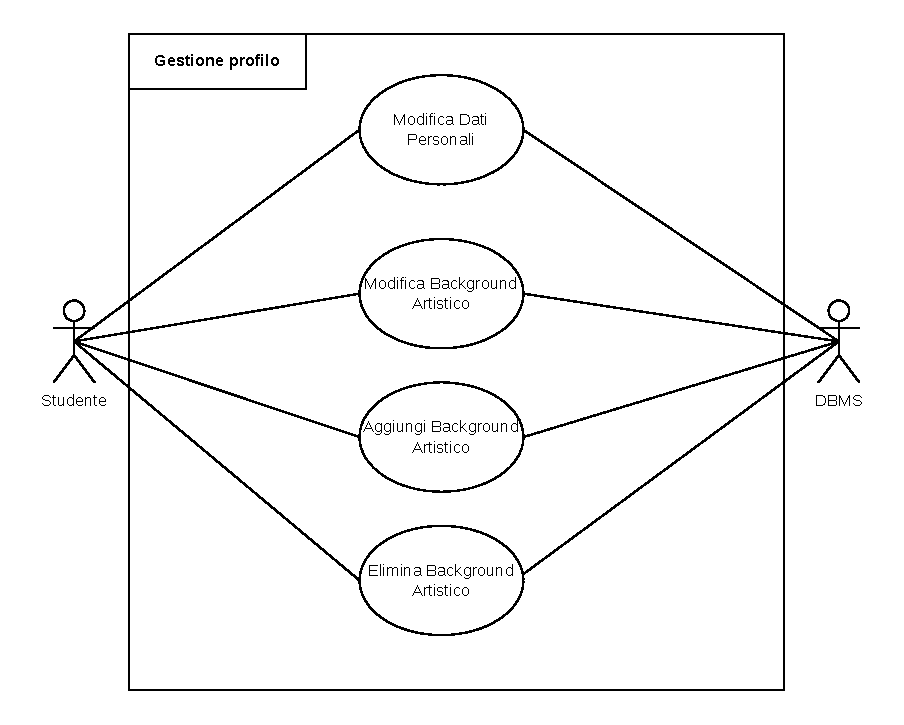
\includegraphics[width=\textwidth,height=1.2\textheight,keepaspectratio]{pdf/GestioneProfilo/Gestione profilo.pdf}
    \caption{Vista d'insieme di Gestione Profilo}
    \label{fig:gestione_prof}
\end{figure}

\newpage
\subparagraph{Modifica Dati Personali}

Questo caso d'uso descrive la procedura con cui lo studente consulta e modifica i propri dati personali.

\footnotesize
\begin{longtable}{|
>{\columncolor{unipablue}\color{white}\bfseries\raggedright\arraybackslash}p{3.4cm}|
>{\raggedright\arraybackslash}p{10.2cm}|}
\hline
Caso d’uso & Modifica Dati Personali \\ \hline
ID & 2.1 \\ \hline
Attori & Studente (iniziatore), DBMS (partecipante) \\ \hline
Precondizioni & Il Sistema ha mostrato a schermo la schermata ``Home AFAM''. \\ \hline
Flusso degli eventi &
\begin{enumerate}[topsep=0.2em,itemsep=0.15em,parsep=0pt,partopsep=0pt]
    \item Lo studente clicca sul pulsante ``Gestione Profilo''.
    \item Il Sistema mostra a video la schermata ``Gestione Profilo''.
    \item Lo studente clicca sul pulsante ``Dati Personali''.
    \item Il Sistema recupera dalla memoria i dati dello studente.
    \item Il Sistema mostra a video la schermata ``Dati Personali'' contenente i dati dello studente (Nome, Cognome, Foto, E-mail e Numero di telefono) e il pulsante ``Modifica Dati''.
    \item Lo studente clicca sul pulsante ``Modifica Dati''.
    \item Il Sistema mostra a video il form di modifica dei dati personali con i campi editabili.
\end{enumerate} \\
&
\begin{enumerate}[topsep=0pt,itemsep=0.15em,parsep=0pt,partopsep=0pt]
    \setcounter{enumi}{7}
    \item Lo studente inserisce i nuovi dati.
    \item Lo studente clicca sul pulsante ``Conferma Modifiche''.
    \item Il Sistema invia i nuovi dati aggiornati al DBMS per la sovrascrittura permanente sul database.
    \item Il Sistema aggiorna i dati dello studente in memoria.
    \item Il Sistema mostra a video il messaggio di conferma: ``Modifiche effettuate correttamente''.
    \item Lo studente clicca sul pulsante ``ok'' per chiudere il messaggio.
    \item Il Sistema mostra nuovamente la schermata ``Dati Personali'', aggiornata con i nuovi valori.
\end{enumerate} \\ \hline
Postcondizioni &
\begin{enumerate}[topsep=0.2em,itemsep=0.15em,parsep=0pt,partopsep=0pt]
    \item Il Sistema ha mostrato la schermata ``Dati Personali''.
\end{enumerate} \\ \hline
Requisiti speciali &
\begin{itemize}[topsep=0.2em,itemsep=0.15em,parsep=0pt,partopsep=0pt]
    \item La nuova e-mail deve contenere una ``@'' e almeno un ``.''.
    \item Il numero di telefono deve contenere esclusivamente caratteri numerici.
    \item Il numero di telefono deve contenere esattamente 10 caratteri.
    \item La foto deve avere formato PNG o JPG.
\end{itemize} \\ \hline
\caption{Scheda di dettaglio del Caso d'Uso Modifica Dati Personali}
\label{tab:uc_modifica_dati_personali}\\
\end{longtable}
\normalsize



\newpage
\subparagraph{Modifica Background Artistico}

Questo caso d'uso descrive la procedura con cui lo studente modifica un'informazione già presente nel proprio background artistico.

\small
\begin{longtable}{|
>{\columncolor{unipablue}\color{white}\bfseries\raggedright\arraybackslash}p{3.4cm}|
>{\raggedright\arraybackslash}p{10.2cm}|}
\hline
Caso d’uso & Modifica Background Artistico \\ \hline
ID & 2.2 \\ \hline
Attori & Studente (iniziatore), DBMS (partecipante) \\ \hline
Precondizioni & Il Sistema ha mostrato a video la schermata ``BackgroundArtistico'' e ha recuperato i dati dello studente. \\ \hline
Flusso degli eventi &
\begin{enumerate}
    \item Lo studente clicca sul pulsante ``Modifica Dati'' relativo all'informazione.
    \item Il Sistema mostra a video il form di modifica del background artistico con i campi editabili.
    \item Lo studente inserisce i nuovi dati.
    \item Lo studente clicca sul pulsante ``Conferma Modifiche''.
    \item Il Sistema invia i nuovi dati aggiornati al DBMS per la sovrascrittura permanente sul database.
    \item Il Sistema aggiorna i dati dello studente in memoria.
    \item Il Sistema mostra a video il messaggio di conferma: ``Modifiche effettuate correttamente''.
    \item Lo studente clicca sul pulsante ``ok'' per chiudere il messaggio.
    \item Il Sistema mostra nuovamente la schermata ``BackgroundArtistico'', aggiornata con i nuovi valori.
\end{enumerate} \\ \hline
Postcondizioni &
\begin{enumerate}
    \item Il Sistema ha mostrato la schermata ``BackgroundArtistico''.
\end{enumerate} \\ \hline
Requisiti speciali &
\begin{itemize}
    \item I campi di testo per l'inserimento della scuola o università frequentata, delle collaborazioni fatte, delle collaborazioni con autori e delle partecipazioni devono avere una lunghezza massima di 700 caratteri.
\end{itemize} \\ \hline
\caption{Scheda di dettaglio del Caso d'Uso Modifica Background Artistico}
\label{tab:uc_modifica_background_artistico}\\
\end{longtable}
\normalsize

\newpage
\subparagraph{Aggiungi Background Artistico}

Questo caso d'uso descrive la procedura con cui lo studente aggiunge nuove informazioni al proprio background artistico.

\footnotesize
\begin{longtable}{|
>{\columncolor{unipablue}\color{white}\bfseries\raggedright\arraybackslash}p{3.4cm}|
>{\raggedright\arraybackslash}p{10.2cm}|}
\hline
Caso d’uso & Aggiungi Background Artistico \\ \hline
ID & 2.3 \\ \hline
Attori & Studente (iniziatore), DBMS (partecipante) \\ \hline
Precondizioni & Il Sistema ha mostrato a schermo la schermata ``Home AFAM''. \\ \hline
Flusso degli eventi &
\begin{enumerate}[topsep=0.2em,itemsep=0.15em,parsep=0pt,partopsep=0pt]
    \item Lo studente clicca sul pulsante ``Gestione Profilo''.
    \item Il Sistema mostra a video la schermata ``Gestione Profilo''.
    \item Lo studente clicca sul pulsante ``BACKGROUND ARTISTICO''.
    \item Il Sistema recupera dalla memoria i dati dello studente.
    \item Il Sistema mostra a video la schermata ``BackgroundArtistico'', contenente i dati attuali dello studente (Scuola/Università frequentata, Collaborazioni fatte, Collaborazioni con autori e Partecipazioni).
    \item Lo studente clicca sul pulsante ``Aggiungi Dati''.
    \item Il Sistema mostra a video il form di aggiunta del background artistico con i campi editabili.
\end{enumerate} \\
&
\begin{enumerate}[topsep=0pt,itemsep=0.15em,parsep=0pt,partopsep=0pt]
    \setcounter{enumi}{7}
    \item Lo studente inserisce i nuovi dati.
    \item Lo studente clicca sul pulsante ``Conferma''.
    \item Il Sistema invia i nuovi dati al DBMS per la sovrascrittura permanente sul database.
    \item Il Sistema aggiorna i dati dello studente in memoria.
    \item Il Sistema mostra a video il messaggio di conferma: ``Aggiunto nuovo background''.
    \item Lo studente clicca sul pulsante ``ok'' per chiudere il messaggio.
    \item Il Sistema mostra nuovamente la schermata ``BackgroundArtistico'', aggiornata con i nuovi valori.
\end{enumerate} \\ \hline
Postcondizioni &
\begin{enumerate}[topsep=0.2em,itemsep=0.15em,parsep=0pt,partopsep=0pt]
    \item Il Sistema ha mostrato la schermata ``BackgroundArtistico''.
\end{enumerate} \\ \hline
Requisiti speciali &
\begin{itemize}[topsep=0.2em,itemsep=0.15em,parsep=0pt,partopsep=0pt]
    \item I campi di testo per l'inserimento della scuola o università frequentata, delle collaborazioni fatte, delle collaborazioni con autori e delle partecipazioni devono avere una lunghezza massima di 700 caratteri.
\end{itemize} \\ \hline
\caption{Scheda di dettaglio del Caso d'Uso Aggiungi Background Artistico}
\label{tab:uc_aggiungi_background_artistico}\\
\end{longtable}
\normalsize

\newpage
\subparagraph{Elimina Background Artistico}

Questo caso d'uso descrive la procedura con cui lo studente elimina un'informazione dal proprio background artistico.

\small
\begin{longtable}{|
>{\columncolor{unipablue}\color{white}\bfseries\raggedright\arraybackslash}p{3.4cm}|
>{\raggedright\arraybackslash}p{10.2cm}|}
\hline
Caso d’uso & Elimina Background Artistico \\ \hline
ID & 2.4 \\ \hline
Attori & Studente (iniziatore), DBMS (partecipante) \\ \hline
Precondizioni & Il Sistema ha mostrato a video la schermata ``BackgroundArtistico'' e ha recuperato i dati dello studente. \\ \hline
Flusso degli eventi &
\begin{enumerate}
    \item Lo studente clicca sul pulsante ``Elimina Dati'' relativo all'informazione.
    \item Il Sistema mostra a video il messaggio di avviso: ``Sei sicuro di eliminare questa informazione?''.
    \item Lo studente clicca sul pulsante ``ok''.
    \item Il Sistema invia i nuovi dati aggiornati al DBMS per la sovrascrittura permanente sul database.
    \item Il Sistema aggiorna i dati dello studente in memoria.
    \item Il Sistema mostra nuovamente la schermata ``BackgroundArtistico'', aggiornata con i nuovi valori.
\end{enumerate} \\ \hline
Postcondizioni &
\begin{enumerate}
    \item Il Sistema ha mostrato la schermata ``BackgroundArtistico''.
\end{enumerate} \\ \hline
\caption{Scheda di dettaglio del Caso d'Uso Elimina Background Artistico}
\label{tab:uc_elimina_background_artistico}\\
\end{longtable}
\normalsize

\newpage 

\paragraph{Caso d'uso : Gestione Contenuti}
All’interno della suddetta macro-categoria sono presenti i seguenti casi d’uso di dettaglio:
\begin{itemize}[topsep=0.25em,itemsep=0.1em,parsep=0pt,partopsep=0pt]
    \item \textbf{Seleziona Categoria Artistica (3.1):}
    \item \textbf{Crea Categoria Artistica (3.2):}
    \item \textbf{Seleziona Tipologia File (3.3):}
    \item \textbf{Upload file (3.4):} 
    \item \textbf{Elimina file (3.5):} 
    \item \textbf{Modifica file (3.6):} 
    \item \textbf{Gestisci privacy contenuti (3.7):} 

\end{itemize}

\vspace{-0.5em}
\begin{figure}[H]
    \centering
    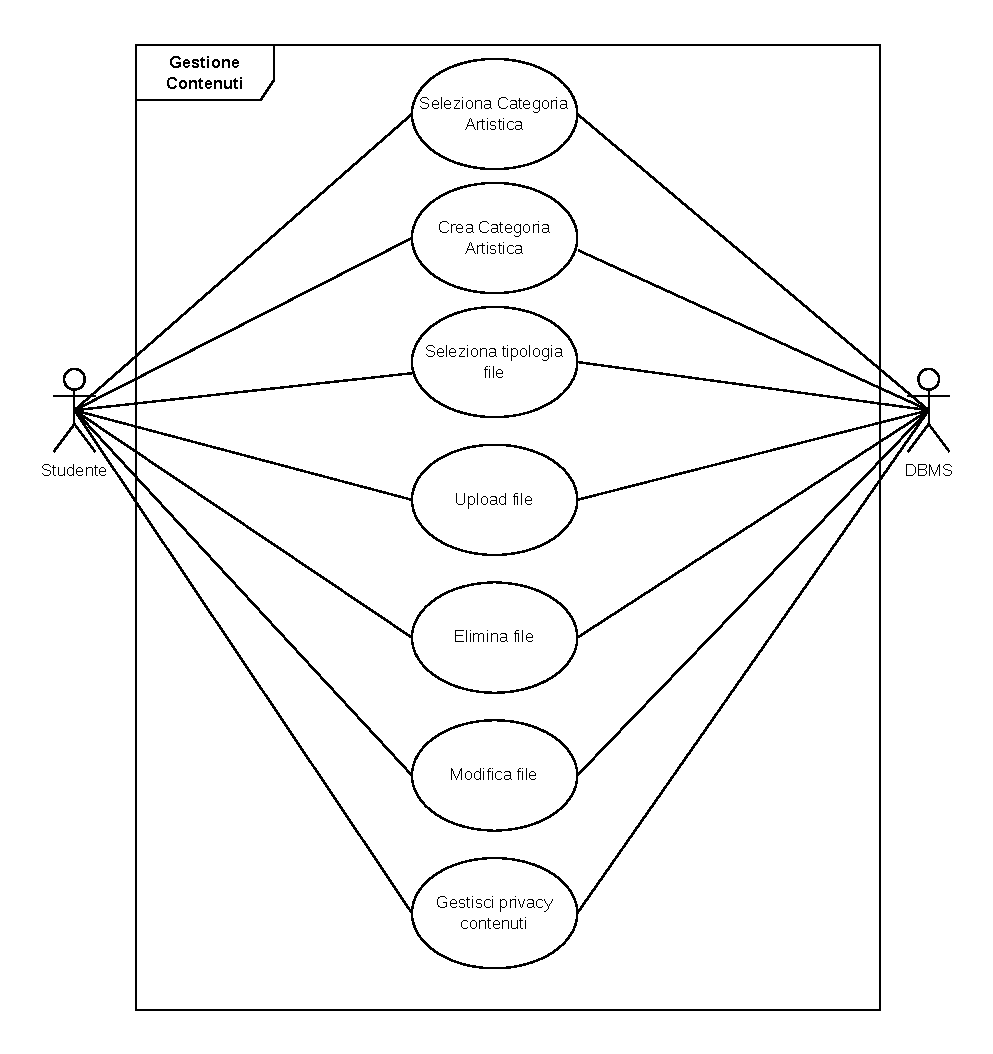
\includegraphics[width=1.2\textwidth,height=0.58\textheight,keepaspectratio]{pdf/GestioneContenuti/GestioneContenuti.pdf}
    \captionsetup{skip=3pt}
    \caption{Vista d'insieme di Gestione Contenuti}
    \label{fig:gestione_cont}
\end{figure}

\newpage
\subparagraph{Seleziona Categoria Artistica}

Questo caso d'uso descrive la procedura con cui lo studente seleziona una categoria artistica associata al proprio profilo.

\small
\begin{longtable}{|
>{\columncolor{unipablue}\color{white}\bfseries\raggedright\arraybackslash}p{3.4cm}|
>{\raggedright\arraybackslash}p{10.2cm}|}
\hline
Caso d’uso & Seleziona Categoria Artistica \\ \hline
ID & 3.1 \\ \hline
Attori & Studente (iniziatore), DBMS (partecipante) \\ \hline
Precondizioni & Il Sistema ha mostrato a schermo la schermata ``Home AFAM''. \\ \hline
Flusso degli eventi &
\begin{enumerate}
    \item Lo studente clicca sul pulsante ``Gestione Contenuti''.
    \item Il Sistema recupera dalla memoria temporanea l'identificativo dello studente.
    \item Il Sistema interroga il DBMS per recuperare la lista delle Categorie Artistiche (es. Pianoforte, Danza Classica, Pittura) associate allo studente.
    \item Il Sistema mostra a video la schermata ``Gestione Contenuti'', elencando le Categorie Artistiche esistenti e il pulsante ``Crea Nuova Categoria Artistica''.
    \item Lo studente clicca sulla Categoria Artistica desiderata.
    \item Il Sistema mostra a video la schermata ``Scelta Tipologia File'' relativa a quella categoria.
\end{enumerate} \\ \hline
Postcondizioni &
\begin{enumerate}
    \item Il Sistema ha mostrato a schermo la schermata per la scelta della tipologia dei file.
\end{enumerate} \\ \hline
\caption{Scheda di dettaglio del Caso d'Uso Seleziona Categoria Artistica}
\label{tab:uc_seleziona_categoria_artistica}\\
\end{longtable}
\normalsize

\newpage
\subparagraph{Crea Categoria Artistica}

Questo caso d'uso descrive la procedura con cui lo studente crea una nuova categoria artistica.

\footnotesize
\begin{longtable}{|
>{\columncolor{unipablue}\color{white}\bfseries\raggedright\arraybackslash}p{3.4cm}|
>{\raggedright\arraybackslash}p{10.2cm}|}
\hline
Caso d’uso & Crea Categoria Artistica \\ \hline
ID & 3.2 \\ \hline
Attori & Studente (iniziatore), DBMS (partecipante) \\ \hline
Precondizioni & Il Sistema ha mostrato a schermo la schermata ``Home AFAM''. \\ \hline
Flusso degli eventi &
\begin{enumerate}[topsep=0.2em,itemsep=0.15em,parsep=0pt,partopsep=0pt]
    \item Lo studente clicca sul pulsante ``Gestione Contenuti''.
    \item Il Sistema recupera dalla memoria temporanea l'identificativo dello studente.
    \item Il Sistema interroga il DBMS per recuperare la lista delle Categorie Artistiche associate allo studente.
    \item Il Sistema mostra a video la schermata ``Gestione Contenuti'', elencando le Categorie Artistiche esistenti e il pulsante ``Crea Nuova Categoria Artistica''.
    \item Lo studente clicca sul pulsante ``Crea Nuova Categoria Artistica''.
    \item Il Sistema mostra a video il form di inserimento ``Nuova Categoria Artistica''.
    \item Lo studente inserisce il nome della nuova Categoria Artistica e clicca sul pulsante ``Salva''.
    \item Il Sistema invia il nome della nuova Categoria Artistica al DBMS per il salvataggio permanente.
    \item Il Sistema mostra a video il messaggio di conferma ``Categoria Artistica creata con successo''.
    \item Lo studente clicca sul pulsante ``ok'' per chiudere il messaggio.
    \item Il Sistema mostra a video la schermata ``Scelta Tipologia File'' relativa alla categoria appena creata.
\end{enumerate} \\ \hline
Postcondizioni &
\begin{enumerate}[topsep=0.2em,itemsep=0.15em,parsep=0pt,partopsep=0pt]
    \item Il Sistema ha mostrato a schermo la schermata per la scelta della tipologia dei file.
\end{enumerate} \\ \hline
Requisiti speciali &
\begin{enumerate}[topsep=0.2em,itemsep=0.15em,parsep=0pt,partopsep=0pt]
    \item Il campo dove inserire il nome della categoria artistica non può essere vuoto.
    \item Il nome della categoria artistica deve essere univoco.
\end{enumerate} \\ \hline
\caption{Scheda di dettaglio del Caso d'Uso Crea Categoria Artistica}
\label{tab:uc_crea_categoria_artistica}\\
\end{longtable}
\normalsize

\newpage
\subparagraph{Seleziona Tipologia File}

Questo caso d'uso descrive la procedura con cui lo studente seleziona una tipologia di file da consultare.

\small
\begin{longtable}{|
>{\columncolor{unipablue}\color{white}\bfseries\raggedright\arraybackslash}p{3.4cm}|
>{\raggedright\arraybackslash}p{10.2cm}|}
\hline
Caso d’uso & Seleziona Tipologia File \\ \hline
ID & 3.3 \\ \hline
Attori & Studente (iniziatore), DBMS (partecipante) \\ \hline
Precondizioni & Il Sistema ha mostrato a schermo la schermata per la scelta della tipologia dei file. \\ \hline
Flusso degli eventi &
\begin{enumerate}
    \item Lo studente seleziona la tipologia di file di interesse cliccando sul relativo pulsante.
    \item Il Sistema interroga il DBMS per recuperare i dati relativi ai file appartenenti alla tipologia selezionata.
    \item Il Sistema mostra a video la schermata contenente l'elenco dei file disponibili per la tipologia scelta.
\end{enumerate} \\ \hline
Postcondizioni &
\begin{enumerate}
    \item Il Sistema ha mostrato a schermo la schermata contenente i file.
\end{enumerate} \\ \hline
\caption{Scheda di dettaglio del Caso d'Uso Seleziona Tipologia File}
\label{tab:uc_seleziona_tipologia_file}\\
\end{longtable}
\normalsize

\newpage
\subparagraph{Upload File}

Questo caso d'uso descrive la procedura con cui lo studente carica un nuovo file nella tipologia selezionata.

\footnotesize
\begin{longtable}{|
>{\columncolor{unipablue}\color{white}\bfseries\raggedright\arraybackslash}p{3.4cm}|
>{\raggedright\arraybackslash}p{10.2cm}|}
\hline
Caso d’uso & Upload File \\ \hline
ID & 3.4 \\ \hline
Attori & Studente (iniziatore), DBMS (partecipante) \\ \hline
Precondizioni & Il Sistema ha mostrato a schermo la schermata contenente i file. \\ \hline
Flusso degli eventi &
\begin{enumerate}[topsep=0.2em,itemsep=0.15em,parsep=0pt,partopsep=0pt]
    \item Lo studente clicca sul pulsante ``UPLOAD''.
    \item Il Sistema mostra a video la Schermata di Caricamento contenente i campi ``Titolo'', ``Descrizione'', il pulsante ``Scegli File'' e il pulsante ``Conferma''.
    \item Lo studente compila i campi ``Titolo'' e ``Descrizione''.
    \item Lo studente clicca su ``Scegli File'', seleziona il file dal proprio dispositivo e lo allega.
    \item Lo studente clicca sul pulsante ``Conferma''.
    \item Il Sistema verifica le dimensioni del file associato.
    \item \textbf{SE} supera le dimensioni massime:
    \begin{itemize}[topsep=0.15em,itemsep=0.1em,parsep=0pt,partopsep=0pt]
        \item[7.1.] Il Sistema mostra a schermo il messaggio di errore: ``File troppo grande''.
        \item[7.2.] Lo studente clicca su ``OK''.
        \item[7.3.] Il Sistema mostra a schermo la schermata contenente i file.
    \end{itemize}
\end{enumerate} \\
&
\begin{enumerate}[topsep=0pt,itemsep=0.15em,parsep=0pt,partopsep=0pt]
    \setcounter{enumi}{7}
    \item \textbf{ALTRIMENTI} (dimensioni massime non superate):
    \begin{itemize}[topsep=0.15em,itemsep=0.1em,parsep=0pt,partopsep=0pt]
        \item[8.1.] Il Sistema recupera dalla memoria temporanea l'identificativo dello studente.
        \item[8.2.] Il Sistema memorizza il contenuto all'interno del DBMS.
        \item[8.3.] Il Sistema mostra a schermo il messaggio: ``File caricato con successo''.
        \item[8.4.] Lo studente clicca su ``OK''.
        \item[8.5.] Il Sistema mostra la schermata contenente i file.
    \end{itemize}
\end{enumerate} \\ \hline
Postcondizioni & Il Sistema ha mostrato a schermo la schermata contenente i file. \\ \hline
Requisiti speciali &
\begin{enumerate}[topsep=0.2em,itemsep=0.15em,parsep=0pt,partopsep=0pt]
    \item Il campo di testo per il titolo non può essere vuoto.
    \item Il campo di testo per il titolo può contenere al massimo 200 caratteri.
    \item I file caricati non devono superare 1 GB di dimensione.
    \item I file caricati devono avere formato idoneo alla categoria selezionata (es. MP4 per i video, PNG per le immagini, MP3 per i file audio).
\end{enumerate} \\ \hline
\caption{Scheda di dettaglio del Caso d'Uso Upload File}
\label{tab:uc_upload_file}\\
\end{longtable}
\normalsize

\newpage
\subparagraph{Elimina File}

Questo caso d'uso descrive la procedura con cui lo studente elimina un file dalla tipologia selezionata.

\small
\begin{longtable}{|
>{\columncolor{unipablue}\color{white}\bfseries\raggedright\arraybackslash}p{3.4cm}|
>{\raggedright\arraybackslash}p{10.2cm}|}
\hline
Caso d’uso & Elimina File \\ \hline
ID & 3.5 \\ \hline
Attori & Studente (iniziatore), DBMS (partecipante) \\ \hline
Precondizioni & Il Sistema ha mostrato a schermo la schermata contenente i file. \\ \hline
Flusso degli eventi &
\begin{enumerate}
    \item Lo studente clicca su ``+'' accanto al file di interesse.
    \item Il Sistema mostra un menu a tendina con varie voci.
    \item Lo studente seleziona la voce ``ELIMINA FILE''.
    \item Il Sistema mostra a schermo una finestra contenente un messaggio in cui si richiede la conferma dell'azione, specificando che sarà irreversibile, e un pulsante ``Conferma''.
    \item Lo studente clicca sul pulsante ``Conferma''.
    \item Il Sistema recupera dalla memoria temporanea l'identificativo dello studente.
    \item Il Sistema aggiorna il DBMS eliminando il file.
    \item Il Sistema mostra a schermo il messaggio ``File eliminato correttamente''.
    \item Lo studente clicca sul pulsante ``OK''.
    \item Il Sistema mostra a schermo la schermata contenente i file.
\end{enumerate} \\ \hline
Postcondizioni & Il Sistema ha mostrato a schermo la schermata contenente i file. \\ \hline
\caption{Scheda di dettaglio del Caso d'Uso Elimina File}
\label{tab:uc_elimina_file}\\
\end{longtable}
\normalsize

\newpage
\subparagraph{Modifica File}

Questo caso d'uso descrive la procedura con cui lo studente modifica un file già presente.

\small
\begin{longtable}{|
>{\columncolor{unipablue}\color{white}\bfseries\raggedright\arraybackslash}p{3.4cm}|
>{\raggedright\arraybackslash}p{10.2cm}|}
\hline
Caso d’uso & Modifica File \\ \hline
ID & 3.6 \\ \hline
Attori & Studente (iniziatore), DBMS (partecipante) \\ \hline
Precondizioni & Il Sistema ha mostrato a schermo la schermata contenente i file. \\ \hline
Flusso degli eventi &
\begin{enumerate}
    \item Lo studente clicca su ``+'' accanto al file di interesse.
    \item Il Sistema mostra a schermo un menu a tendina con varie voci.
    \item Lo studente seleziona la voce ``MODIFICA FILE''.
    \item Il Sistema mostra a schermo il form contenente file, descrizione e titolo attuali del file selezionato e un pulsante ``Conferma Modifica''.
    \item Lo studente effettua le modifiche desiderate all'interno del form.
    \item Lo studente clicca sul pulsante ``CONFERMA MODIFICA''.
    \item Il Sistema recupera dalla memoria temporanea l'identificativo dello studente.
    \item Il Sistema invia i nuovi dati inseriti al DBMS.
    \item Il Sistema mostra a video il messaggio di conferma: ``Modifica effettuata correttamente''.
    \item Lo studente clicca sul pulsante ``OK''.
    \item Il Sistema mostra a schermo la schermata contenente i file.
\end{enumerate} \\ \hline
Postcondizioni & Il Sistema ha mostrato a schermo la schermata contenente i file. \\ \hline
\caption{Scheda di dettaglio del Caso d'Uso Modifica File}
\label{tab:uc_modifica_file}\\
\end{longtable}
\normalsize

\newpage
\subparagraph{Gestisci Privacy Contenuti}

Questo caso d'uso descrive la procedura con cui lo studente modifica le impostazioni di privacy di un file.

\small
\begin{longtable}{|
>{\columncolor{unipablue}\color{white}\bfseries\raggedright\arraybackslash}p{3.4cm}|
>{\raggedright\arraybackslash}p{10.2cm}|}
\hline
Caso d’uso & Gestisci Privacy Contenuti \\ \hline
ID & 3.7 \\ \hline
Attori & Studente (iniziatore), DBMS (partecipante) \\ \hline
Precondizioni & Il Sistema ha mostrato a schermo la schermata contenente i file. \\ \hline
Flusso degli eventi &
\begin{enumerate}
    \item Lo studente clicca su ``+'' accanto al file di interesse.
    \item Il Sistema mostra a schermo un menu a tendina con varie voci.
    \item Lo studente seleziona la voce ``PRIVACY''.
    \item Il Sistema mostra a video la schermata ``Modifica Privacy'' contenente le opzioni di visualizzazione del file (Pubblico, Privato) e il pulsante ``Conferma Modifica''.
    \item Lo studente seleziona l'opzione desiderata.
    \item Lo studente clicca sul pulsante ``CONFERMA MODIFICA''.
    \item Il Sistema recupera dalla memoria temporanea l'identificativo dello studente.
    \item Il Sistema invia la nuova impostazione di privacy al DBMS.
    \item Il Sistema mostra a video il messaggio di conferma: ``Impostazioni di privacy aggiornate correttamente''.
    \item Lo studente clicca sul pulsante ``OK'' per chiudere il messaggio.
    \item Il Sistema mostra a video la schermata contenente i file.
\end{enumerate} \\ \hline
Postcondizioni & Il Sistema ha mostrato a schermo la schermata contenente i file. \\ \hline
\caption{Scheda di dettaglio del Caso d'Uso Gestisci Privacy Contenuti}
\label{tab:uc_gestisci_privacy_contenuti}\\
\end{longtable}
\normalsize

\newpage
\paragraph{Caso d'uso : Gestione Condivisione con Link}
All’interno della suddetta macro-categoria sono presenti i seguenti casi d’uso di dettaglio:
\begin{itemize}[topsep=0.25em,itemsep=0.1em,parsep=0pt,partopsep=0pt]
    \item \textbf{Seleziona contenuti (4.1):}
    \item \textbf{Genera link (4.2):}
    \item \textbf{Visualizza Elenco Link (4.3):}
    \item \textbf{Revoca Link (4.4):}
    \item \textbf{Verifica Validità Link (4.5):}

\end{itemize}

\begin{figure}[H]
    \centering
    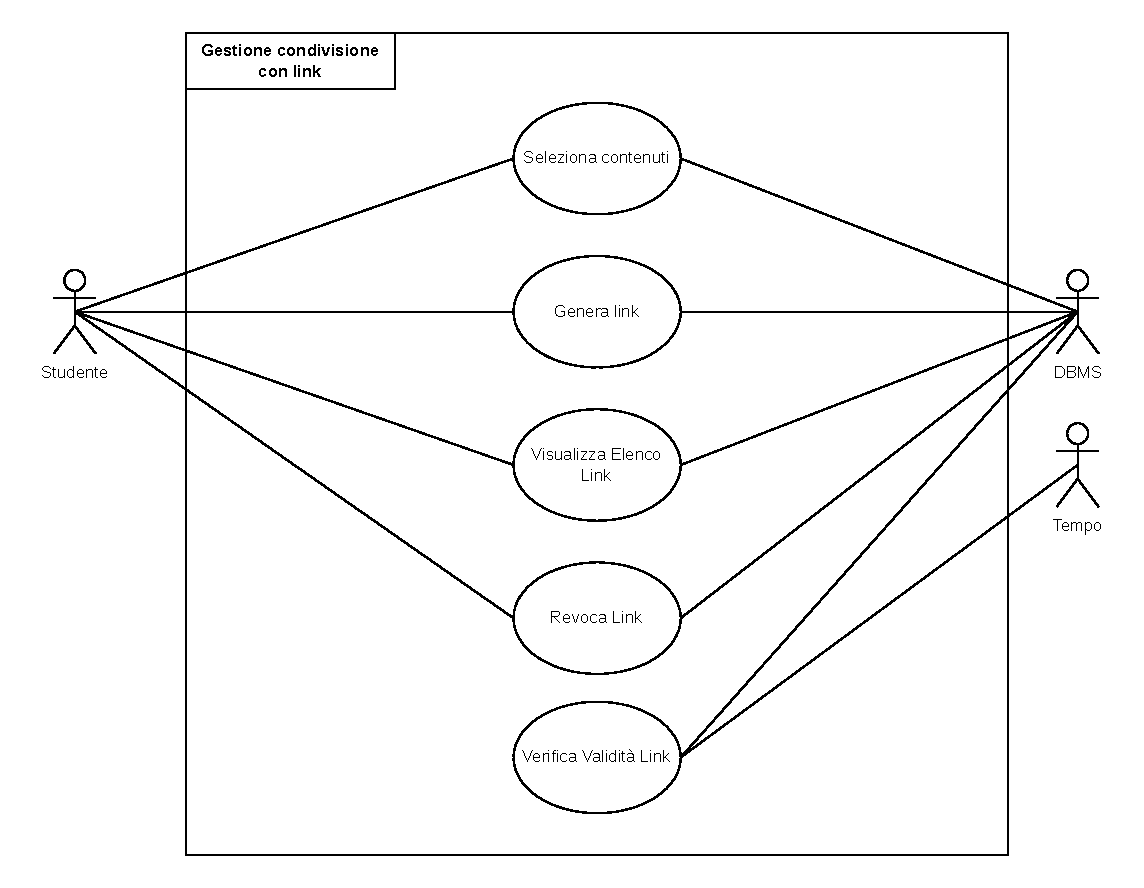
\includegraphics[width=\textwidth,height=1.2\textheight,keepaspectratio]{pdf/GestioneCondLink/Gestcondivisioneconlink.pdf}
    \caption{Vista d'insieme di Gestione Condivisione con Link}
    \label{fig:gestione_condLink}
\end{figure}

\newpage

\subparagraph{Selezione Contenuti}

Questo caso d'uso descrive la procedura con cui lo studente seleziona i contenuti da condividere tramite link.

\footnotesize
\begin{longtable}{|
>{\columncolor{unipablue}\color{white}\bfseries\raggedright\arraybackslash}p{3.4cm}|
>{\raggedright\arraybackslash}p{10.2cm}|}
\hline
Caso d’uso & Selezione Contenuti \\ \hline
ID & 4.1 \\ \hline
Attori & Studente (iniziatore), DBMS (partecipante) \\ \hline
Precondizioni & Il Sistema ha mostrato a video la schermata ``Home AFAM''. \\ \hline
Flusso degli eventi &
\begin{enumerate}[topsep=0.2em,itemsep=0.15em,parsep=0pt,partopsep=0pt]
    \item Lo studente clicca sulla sezione ``Gestione condivisione tramite link''.
    \item Il Sistema mostra a video la schermata ``Gestione Condivisione tramite Link''.
    \item Lo studente clicca sul pulsante ``Seleziona Contenuti''.
    \item Il Sistema recupera dalla memoria temporanea l'identificativo dello studente.
    \item Il Sistema interroga il DBMS per recuperare la struttura dei contenuti (strumenti e file).
    \item \textbf{SE} lo studente non ha alcun contenuto caricato:
    \begin{itemize}[topsep=0.15em,itemsep=0.1em,parsep=0pt,partopsep=0pt]
        \item[6.1.] Il Sistema mostra a video il messaggio di errore: ``Nessun contenuto disponibile''.
        \item[6.2.] Lo studente clicca sul pulsante ``ok'' per chiuderlo.
        \item[6.3.] Il Sistema mostra nuovamente la schermata ``Gestione Condivisione tramite Link''.
    \end{itemize}
    \item \textbf{ALTRIMENTI} (ci sono contenuti disponibili):
    \begin{itemize}[topsep=0.15em,itemsep=0.1em,parsep=0pt,partopsep=0pt]
        \item[7.1.] Il Sistema mostra a video la schermata ``Seleziona Contenuti'', contenente l'elenco dei contenuti suddivisi per categoria e il pulsante ``Conferma Selezione Finale''.
        \item[7.2.] Lo studente seleziona i contenuti desiderati.
        \item[7.3.] Lo studente clicca sul pulsante ``Conferma Selezione Finale''.
        \item[7.4.] Il Sistema mostra a video la schermata ``Generazione Link''.
    \end{itemize}
\end{enumerate} \\ \hline
Postcondizioni &
\begin{enumerate}[topsep=0.2em,itemsep=0.15em,parsep=0pt,partopsep=0pt]
    \item Il Sistema ha mostrato a video la schermata ``Generazione Link''.
    \item Il Sistema ha mostrato la schermata ``Gestione Condivisione tramite Link''.
\end{enumerate} \\ \hline
Note &
\begin{minipage}[t]{\linewidth}
I contenuti sono organizzati secondo una struttura gerarchica a due livelli:
\begin{enumerate}[topsep=0.2em,itemsep=0.15em,parsep=0pt,partopsep=0pt]
    \item \textbf{Livello primario:} raggruppamento per Argomento Artistico.
    \item \textbf{Livello secondario:} suddivisione per Tipologia di File.
\end{enumerate}
\end{minipage} \\ \hline
\caption{Scheda di dettaglio del Caso d'Uso Selezione Contenuti}
\label{tab:uc_selezione_contenuti_link}\\
\end{longtable}
\normalsize

\newpage
\subparagraph{Genera Link}

Questo caso d'uso descrive la procedura con cui lo studente genera un link univoco per i file selezionati.

\small
\begin{longtable}{|
>{\columncolor{unipablue}\color{white}\bfseries\raggedright\arraybackslash}p{3.4cm}|
>{\raggedright\arraybackslash}p{10.2cm}|}
\hline
Caso d’uso & Genera Link \\ \hline
ID & 4.2 \\ \hline
Attori & Studente (iniziatore), DBMS (partecipante) \\ \hline
Precondizioni & Il Sistema ha mostrato a video la schermata ``Generazione Link''. \\ \hline
Flusso degli eventi &
\begin{enumerate}
    \item Lo studente clicca sul pulsante ``Genera Link''.
    \item Il Sistema genera un link di condivisione univoco associato ai file selezionati.
    \item Il Sistema invia i dati del link generato, l'elenco dei file associati e l'identificativo dello studente al DBMS per la memorizzazione definitiva.
    \item Il Sistema mostra a video un messaggio di conferma: ``Link generato con successo'', contenente il link testuale creato e i pulsanti ``Copia Link'' e ``ok''.
    \item Lo studente clicca sul pulsante ``Copia Link''.
    \item Il Sistema copia il link generato nel dispositivo dello studente.
    \item Lo studente clicca sul pulsante ``ok'' per chiudere il messaggio di conferma.
    \item Il Sistema mostra a video la schermata ``Gestione Condivisione tramite Link''.
\end{enumerate} \\ \hline
Postcondizioni &
\begin{enumerate}
    \item Il Sistema ha mostrato a video la schermata ``Gestione Condivisione tramite Link''.
\end{enumerate} \\ \hline
\caption{Scheda di dettaglio del Caso d'Uso Genera Link}
\label{tab:uc_genera_link}\\
\end{longtable}
\normalsize

\newpage
\subparagraph{Visualizza Elenco Link}

Questo caso d'uso descrive la procedura con cui lo studente consulta l'elenco dei link generati.

\footnotesize
\begin{longtable}{|
>{\columncolor{unipablue}\color{white}\bfseries\raggedright\arraybackslash}p{3.4cm}|
>{\raggedright\arraybackslash}p{10.2cm}|}
\hline
Caso d’uso & Visualizza Elenco Link \\ \hline
ID & 4.3 \\ \hline
Attori & Studente (iniziatore), DBMS (partecipante) \\ \hline
Precondizioni & Il Sistema ha mostrato a video la schermata ``Gestione Condivisione Link''. \\ \hline
Flusso degli eventi &
\begin{enumerate}[topsep=0.2em,itemsep=0.15em,parsep=0pt,partopsep=0pt]
    \item Lo studente clicca sulla sezione ``Gestisci link''.
    \item Il Sistema recupera dalla memoria temporanea l'identificativo dello studente.
    \item Il Sistema interroga il DBMS per recuperare la lista dei link generati dallo studente e il loro stato di visualizzazione.
    \item \textbf{SE} lo studente non possiede alcun link generato:
    \begin{itemize}[topsep=0.15em,itemsep=0.1em,parsep=0pt,partopsep=0pt]
        \item[4.1.] Il Sistema mostra a video un messaggio di errore: ``Nessun link generato''.
        \item[4.2.] Lo studente clicca sul pulsante ``ok''.
        \item[4.3.] Il Sistema mostra a video la schermata ``Gestione Condivisione Link''.
    \end{itemize}
    \item \textbf{ALTRIMENTI} (ci sono link generati):
    \begin{itemize}[topsep=0.15em,itemsep=0.1em,parsep=0pt,partopsep=0pt]
        \item[5.1.] Il Sistema mostra a video la schermata ``Elenco Link'', contenente l'elenco dei link con un indicatore di avvenuta visualizzazione (es. spunta) e il pulsante ``Revoca''.
    \end{itemize}
\end{enumerate} \\ \hline
Postcondizioni &
\begin{enumerate}[topsep=0.2em,itemsep=0.15em,parsep=0pt,partopsep=0pt]
    \item Il Sistema ha mostrato a schermo la schermata ``Elenco Link''.
    \item Il Sistema ha mostrato a video la schermata ``Gestione Condivisione Link''.
\end{enumerate} \\ \hline
\caption{Scheda di dettaglio del Caso d'Uso Visualizza Elenco Link}
\label{tab:uc_visualizza_elenco_link}\\
\end{longtable}
\normalsize

\newpage
\subparagraph{Revoca Link}

Questo caso d'uso descrive la procedura con cui lo studente revoca un link specifico.

\small
\begin{longtable}{|
>{\columncolor{unipablue}\color{white}\bfseries\raggedright\arraybackslash}p{3.4cm}|
>{\raggedright\arraybackslash}p{10.2cm}|}
\hline
Caso d’uso & Revoca Link \\ \hline
ID & 4.4 \\ \hline
Attori & Studente (iniziatore), DBMS (partecipante) \\ \hline
Precondizioni & Il Sistema ha mostrato a video la schermata ``Elenco Link''. \\ \hline
Flusso degli eventi &
\begin{enumerate}
    \item Lo studente clicca sul pulsante ``Revoca'' in corrispondenza di un link specifico.
    \item Il Sistema mostra a video un messaggio di conferma: ``Sei sicuro di voler revocare questo link?'', con i pulsanti ``Conferma'' e ``Annulla''.
    \item Lo studente clicca su ``Conferma''.
    \item Il Sistema invia la richiesta di revoca al DBMS per aggiornare lo stato del link.
    \item Il Sistema mostra nuovamente la schermata ``Elenco Link''.
\end{enumerate} \\ \hline
Postcondizioni &
\begin{enumerate}
    \item Il Sistema ha mostrato a schermo la schermata ``Elenco Link''.
\end{enumerate} \\ \hline
\caption{Scheda di dettaglio del Caso d'Uso Revoca Link}
\label{tab:uc_revoca_link}\\
\end{longtable}
\normalsize

\newpage
\subparagraph{Verifica Validità Link}

Questo caso d'uso descrive il controllo automatico della validità temporale dei link.

\small
\begin{longtable}{|
>{\columncolor{unipablue}\color{white}\bfseries\raggedright\arraybackslash}p{3.4cm}|
>{\raggedright\arraybackslash}p{10.2cm}|}
\hline
Caso d’uso & Verifica Validità Link \\ \hline
ID & 4.5 \\ \hline
Attori & Tempo (iniziatore), DBMS (partecipante) \\ \hline
Precondizioni & \mbox{} \\ \hline
Flusso degli eventi &
\begin{enumerate}
    \item Il Tempo interroga il Sistema sulla data odierna.
    \item \textbf{SE} l'orario corrisponde alle 00:00:
    \begin{itemize}
        \item[2.1.] Il Sistema interroga il DBMS per recuperare la data di scadenza.
        \item[2.2.] \textbf{SE} la data odierna è maggiore della data di scadenza:
        \begin{itemize}
            \item[2.2.1.] Il Sistema aggiorna il DBMS rendendo il link disattivato.
        \end{itemize}
    \end{itemize}
\end{enumerate} \\ \hline
Postcondizioni & \mbox{} \\ \hline
\caption{Scheda di dettaglio del Caso d'Uso Verifica Validità Link}
\label{tab:uc_verifica_validita_link}\\
\end{longtable}
\normalsize

\newpage
\paragraph{Caso d'uso : Consulta Profilo Studente}
All’interno della suddetta macro-categoria sono presenti i seguenti casi d’uso di dettaglio:
\begin{itemize}[topsep=0.25em,itemsep=0.1em,parsep=0pt,partopsep=0pt]
    \item \textbf{Cerca studente (5.1):}
    \item \textbf{Mostra Contenuti Pubblici (5.2):}
    \item \textbf{Mostra Contenuti Privati (5.3):}
    \item \textbf{Visualizza contenuto (5.4):}

\end{itemize}

\begin{figure}[H]
    \centering
    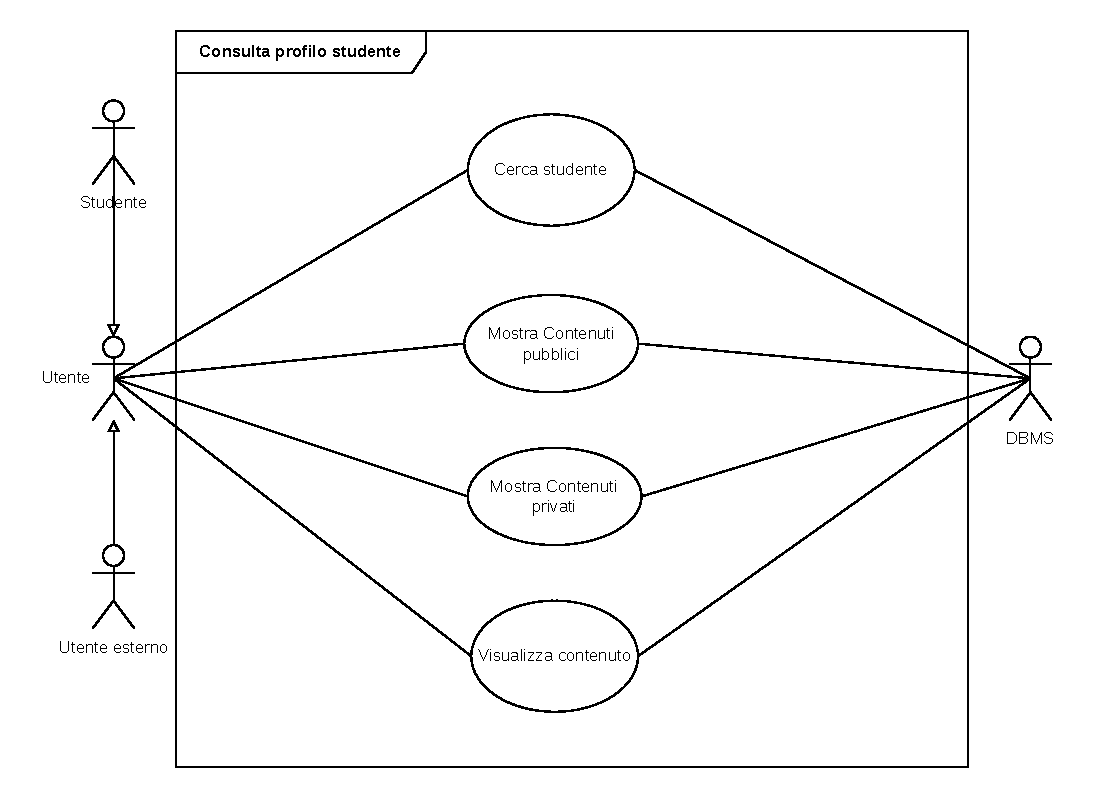
\includegraphics[width=\textwidth,height=1.2\textheight,keepaspectratio]{pdf/ConsultaProfStudente/Consultaprofilostudente.pdf}
    \caption{Vista d'insieme di Consulta Profilo Studente}
    \label{fig:cons_profStud}
\end{figure}

\newpage

\subparagraph{Cerca Studente}

\footnotesize
\begin{longtable}{|
>{\columncolor{unipablue}\color{white}\bfseries\raggedright\arraybackslash}p{3.4cm}|
>{\raggedright\arraybackslash}p{10.2cm}|}
\hline
Caso d'uso & Cerca Studente \\ \hline
ID & 5.1 \\ \hline
Attori & Utente, DBMS \\ \hline
Precondizioni & Il Sistema ha mostrato a schermo la schermata ``Home AFAM''. \\ \hline
Flusso degli eventi &
\begin{enumerate}[topsep=0.2em,itemsep=0.15em,parsep=0pt,partopsep=0pt]
    \item L'utente clicca sul pulsante di ricerca.
    \item Il Sistema mostra a schermo la schermata di ricerca.
    \item L'utente digita il nome e il cognome dello studente da cercare.
    \item L'utente clicca sul pulsante ``INVIO''.
    \item Il Sistema interroga il DBMS per cercare gli studenti corrispondenti.
    \item \textbf{SE} il DBMS restituisce uno o più risultati validi:
    \begin{itemize}[topsep=0.15em,itemsep=0.1em,parsep=0pt,partopsep=0pt]
        \item[6.1.] Il Sistema mostra la schermata ``Risultati Ricerca'' con l'elenco degli studenti trovati.
        \item[6.2.] L'utente clicca sul nome dello studente desiderato.
        \item[6.3.] Il Sistema recupera dal DBMS i dati dello studente selezionato.
        \item[6.4.] Il Sistema mostra la schermata ``Profilo Studente'' con i relativi dettagli.
    \end{itemize}
    \item \textbf{ALTRIMENTI}:
    \begin{itemize}[topsep=0.15em,itemsep=0.1em,parsep=0pt,partopsep=0pt]
        \item[7.1.] Il Sistema mostra il messaggio ``Nessun risultato trovato''.
        \item[7.2.] L'utente clicca sul pulsante ``OK''.
        \item[7.3.] Il Sistema mostra nuovamente la schermata di ricerca.
    \end{itemize}
\end{enumerate} \\ \hline
Postcondizioni &
\begin{enumerate}[topsep=0.2em,itemsep=0.15em,parsep=0pt,partopsep=0pt]
    \item Il Sistema ha mostrato la schermata ``Profilo Studente''.
    \item Il Sistema ha mostrato la schermata di ricerca.
\end{enumerate} \\ \hline
Requisiti speciali & Nel campo di ricerca sono ammessi solo caratteri alfabetici. \\ \hline
\caption{Scheda di dettaglio del Caso d'Uso Cerca Studente}
\label{tab:uc_cerca_studente}\\
\end{longtable}
\normalsize

\newpage
\subparagraph{Mostra Contenuti Pubblici}

\small
\begin{longtable}{|
>{\columncolor{unipablue}\color{white}\bfseries\raggedright\arraybackslash}p{3.4cm}|
>{\raggedright\arraybackslash}p{10.2cm}|}
\hline
Caso d'uso & Mostra Contenuti Pubblici \\ \hline
ID & 5.2 \\ \hline
Attori & Utente, DBMS \\ \hline
Precondizioni & Il Sistema ha mostrato la schermata ``Profilo Studente''. \\ \hline
Flusso degli eventi &
\begin{enumerate}[topsep=0.2em,itemsep=0.15em,parsep=0pt,partopsep=0pt]
    \item L'utente clicca sul pulsante ``Mostra Contenuti Pubblici''.
    \item Il Sistema mostra la schermata ``Contenuti Pubblici''.
    \item Il Sistema recupera dalla memoria l'identificativo dello studente.
    \item L'utente clicca sulla categoria artistica della quale desidera visualizzare i file.
    \item Il Sistema interroga il DBMS per recuperare le tipologie di file disponibili.
    \item Il Sistema mostra la schermata ``Categorie Contenuti'', elencando le tipologie disponibili.
    \item L'utente clicca sulla tipologia desiderata.
    \item Il Sistema interroga il DBMS per recuperare l'elenco dei file caricati per la tipologia selezionata.
    \item Il Sistema mostra la schermata ``Elenco File'' con i risultati.
\end{enumerate} \\ \hline
Postcondizioni & Il Sistema ha mostrato la schermata ``Elenco File''. \\ \hline
\caption{Scheda di dettaglio del Caso d'Uso Mostra Contenuti Pubblici}
\label{tab:uc_mostra_contenuti_pubblici}\\
\end{longtable}
\normalsize

\newpage
\subparagraph{Mostra Contenuti Privati}

\small
\begin{longtable}{|
>{\columncolor{unipablue}\color{white}\bfseries\raggedright\arraybackslash}p{3.4cm}|
>{\raggedright\arraybackslash}p{10.2cm}|}
\hline
Caso d'uso & Mostra Contenuti Privati \\ \hline
ID & 5.3 \\ \hline
Attori & Utente, DBMS \\ \hline
Precondizioni & Il Sistema ha mostrato la schermata "Profilo Studente". \\ \hline
Flusso degli eventi &
\begin{enumerate}[topsep=0.2em,itemsep=0.15em,parsep=0pt,partopsep=0pt]
    \item L'utente clicca sul pulsante ``Visualizza Contenuti Privati''.
    \item Il Sistema recupera dalla memoria l'identificativo dello studente.
    \item Il Sistema mostra la schermata ``Inserimento Codice''.
    \item L'utente inserisce il codice e clicca sul pulsante ``Conferma''.
    \item Il Sistema interroga il DBMS per verificare la validità del codice.
    \item \textbf{SE} il codice non è valido:
    \begin{itemize}[topsep=0.15em,itemsep=0.1em,parsep=0pt,partopsep=0pt]
        \item[6.1.] Il Sistema mostra il messaggio ``Codice errato''.
        \item[6.2.] L'utente clicca sul pulsante ``OK''.
        \item[6.3.] Il Sistema mostra nuovamente la schermata ``Profilo Studente''.
    \end{itemize}
    \item \textbf{ALTRIMENTI}:
    \begin{itemize}[topsep=0.15em,itemsep=0.1em,parsep=0pt,partopsep=0pt]
        \item[7.1.] Il Sistema recupera dalla memoria l'identificativo dello studente.
        \item[7.2.] Il Sistema interroga il DBMS per recuperare l'elenco dei file privati.
        \item[7.3.] Il Sistema mostra la schermata ``Elenco File'' con i risultati.
    \end{itemize}
\end{enumerate} \\ \hline
Postcondizioni &
\begin{enumerate}[topsep=0.2em,itemsep=0.15em,parsep=0pt,partopsep=0pt]
    \item Il Sistema ha mostrato la schermata ``Elenco File''.
    \item Il Sistema ha mostrato la schermata ``Profilo Studente''.
\end{enumerate} \\ \hline
\caption{Scheda di dettaglio del Caso d'Uso Mostra Contenuti Privati}
\label{tab:uc_mostra_contenuti_privati}\\
\end{longtable}
\normalsize

\newpage
\subparagraph{Visualizza Contenuto}

\small
\begin{longtable}{|
>{\columncolor{unipablue}\color{white}\bfseries\raggedright\arraybackslash}p{3.4cm}|
>{\raggedright\arraybackslash}p{10.2cm}|}
\hline
Caso d'uso & Visualizza Contenuto \\ \hline
ID & 5.4 \\ \hline
Attori & Utente, DBMS \\ \hline
Precondizioni & Il Sistema ha mostrato la schermata ``Elenco File'' con i risultati. \\ \hline
Flusso degli eventi &
\begin{enumerate}[topsep=0.2em,itemsep=0.15em,parsep=0pt,partopsep=0pt]
    \item L'utente clicca sul file che desidera visualizzare.
    \item Il Sistema interroga il DBMS per recuperare il file fisico.
    \item Il Sistema controlla il formato del file.
    \item \textbf{SE} il contenuto è multimediale (audio o video):
    \begin{itemize}[topsep=0.15em,itemsep=0.1em,parsep=0pt,partopsep=0pt]
        \item[4.1.] Il Sistema mostra la schermata ``Riproduttore Multimediale'', contenente il lettore e le informazioni del file.
        \item[4.2.] L'utente clicca sul pulsante ``Chiudi Contenuto''.
        \item[4.3.] Il Sistema mostra nuovamente la schermata ``Elenco File''.
    \end{itemize}
    \item \textbf{ALTRIMENTI}, se il contenuto è un documento PDF o un'immagine:
    \begin{itemize}[topsep=0.15em,itemsep=0.1em,parsep=0pt,partopsep=0pt]
        \item[5.1.] Il Sistema mostra la schermata ``Visualizzatore Documenti'', contenente il file e le relative informazioni.
        \item[5.2.] L'utente clicca sul pulsante ``Chiudi Contenuto''.
        \item[5.3.] Il Sistema mostra nuovamente la schermata ``Elenco File''.
    \end{itemize}
\end{enumerate} \\ \hline
Postcondizioni & Il Sistema ha mostrato la schermata ``Elenco File''. \\ \hline
\caption{Scheda di dettaglio del Caso d'Uso Visualizza Contenuto}
\label{tab:uc_visualizza_contenuto}\\
\end{longtable}
\normalsize


\newpage
\paragraph{Caso d'uso : Visualizza Contenuto Tramite Link }
All’interno della suddetta macro-categoria sono presenti i seguenti casi d’uso di dettaglio:
\begin{itemize}[topsep=0.25em,itemsep=0.1em,parsep=0pt,partopsep=0pt]
    \item \textbf{Mostra Contenuti Tramite Link (6.1):}
    \item \textbf{Visualizza Contenuto Tramite Link (6.2):}
 
\end{itemize}

\begin{figure}[H]
    \centering
    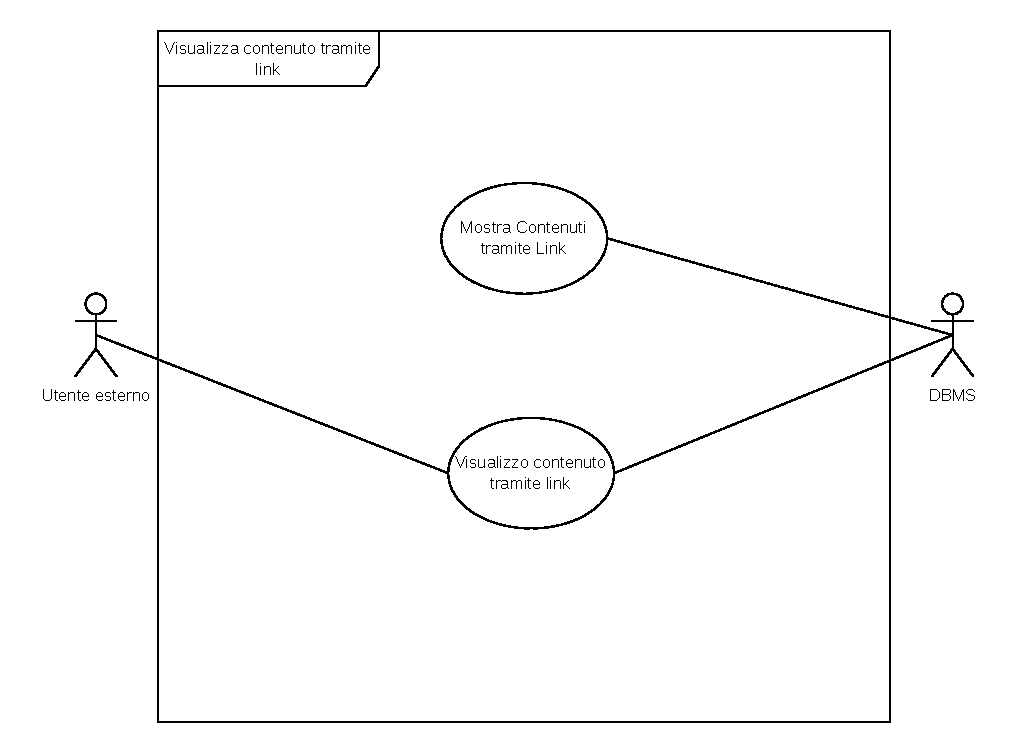
\includegraphics[width=\textwidth,height=1.2\textheight,keepaspectratio]{pdf/VisualizzaContenutoTramiteLink/VistaD'insiemeProgetto-2-Visualizza contenuto con link.drawio.pdf}
    \caption{Vista d'insieme di Visualizza Contenuto Tramite Link}
    \label{fig:visCont_conLink}
\end{figure}

\newpage

\subparagraph{Mostra Contenuti Tramite Link}

\small
\begin{longtable}{|
>{\columncolor{unipablue}\color{white}\bfseries\raggedright\arraybackslash}p{3.4cm}|
>{\raggedright\arraybackslash}p{10.2cm}|}
\hline
Note & Caso particolare. Questo caso d'uso rappresenta un sistema esterno che manda un messaggio al Sistema per trasmettere il link condiviso; per questo si suppone che non ci sia un attore iniziatore. \\ \hline
Caso d'uso & Mostra Contenuti Tramite Link \\ \hline
ID & 6.1 \\ \hline
Attori & DBMS \\ \hline
Precondizioni & \mbox{} \\ \hline
Flusso degli eventi &
\begin{enumerate}[topsep=0.2em,itemsep=0.15em,parsep=0pt,partopsep=0pt]
    \item Il Sistema riceve una richiesta di accesso tramite un link condiviso (\textit{found message}).
    \item Il Sistema estrae il codice univoco dal link.
    \item Il Sistema interroga il DBMS per verificarne lo stato.
    \item \textbf{SE} il link è valido:
    \begin{itemize}[topsep=0.15em,itemsep=0.1em,parsep=0pt,partopsep=0pt]
        \item[4.1.] Il Sistema interroga il DBMS per recuperare l'elenco dei contenuti (file) associati a quel link specifico.
        \item[4.2.] Il Sistema aggiorna lo stato del link nel DBMS per segnalare l'avvenuta visualizzazione.
        \item[4.3.] Il Sistema mostra a video la schermata ``Contenuti Condivisi'', visualizzando l'elenco dei file con i relativi titoli e descrizioni.
    \end{itemize}
\end{enumerate} \\ \hline
Postcondizioni & Il Sistema ha mostrato la schermata ``Contenuti Condivisi''. \\ \hline
\caption{Scheda di dettaglio del Caso d'Uso Mostra Contenuti Tramite Link}
\label{tab:uc_mostra_contenuti_tramite_link}\\
\end{longtable}
\normalsize

\newpage
\subparagraph{Visualizza Contenuto Tramite Link}

\small
\begin{longtable}{|
>{\columncolor{unipablue}\color{white}\bfseries\raggedright\arraybackslash}p{3.4cm}|
>{\raggedright\arraybackslash}p{10.2cm}|}
\hline
Caso d'uso & Visualizza Contenuto Tramite Link \\ \hline
ID & 6.2 \\ \hline
Attori & Utente esterno, DBMS \\ \hline
Precondizioni & Il Sistema ha mostrato la schermata ``Contenuti Condivisi''. \\ \hline
Flusso degli eventi &
\begin{enumerate}[topsep=0.2em,itemsep=0.15em,parsep=0pt,partopsep=0pt]
    \item L'utente clicca su uno specifico file di interesse dall'elenco.
    \item Il Sistema interroga il DBMS per recuperare il file fisico.
    \item Il Sistema controlla il formato del file selezionato.
    \item \textbf{SE} il contenuto è un file multimediale riproducibile, ad esempio una traccia audio o un video:
    \begin{itemize}[topsep=0.15em,itemsep=0.1em,parsep=0pt,partopsep=0pt]
        \item[4.1.] Il Sistema mostra a video la schermata ``Riproduttore Multimediale'', contenente il player attivo e le informazioni descrittive del contenuto.
        \item[4.2.] L'utente clicca sul pulsante ``Chiudi Contenuto''.
        \item[4.3.] Il Sistema mostra la schermata ``Contenuti Condivisi''.
    \end{itemize}
    \item \textbf{ALTRIMENTI} (file PDF o immagini):
    \begin{itemize}[topsep=0.15em,itemsep=0.1em,parsep=0pt,partopsep=0pt]
        \item[5.1.] Il Sistema mostra a video la schermata ``Visualizzatore Documenti'', contenente il file aperto e le informazioni descrittive del contenuto.
        \item[5.2.] L'utente clicca sul pulsante ``Chiudi Contenuto''.
        \item[5.3.] Il Sistema mostra la schermata ``Contenuti Condivisi''.
    \end{itemize}
\end{enumerate} \\ \hline
Postcondizioni & Il Sistema ha mostrato la schermata ``Contenuti Condivisi''. \\ \hline
\caption{Scheda di dettaglio del Caso d'Uso Visualizza Contenuto Tramite Link}
\label{tab:uc_visualizza_contenuto_tramite_link}\\
\end{longtable}
\normalsize


\newpage
\paragraph{Caso d'uso : Gestione Condivisione Interna }
All’interno della suddetta macro-categoria sono presenti i seguenti casi d’uso di dettaglio:
\begin{itemize}[topsep=0.25em,itemsep=0.1em,parsep=0pt,partopsep=0pt]
    \item \textbf{Selezione Contenuti Privati (7.1):}
    \item \textbf{Genera Codice (7.2):}
    \item \textbf{Visualizza Elenco Codici (7.3):}
    \item \textbf{Revoca Codice (7.4):}
 
\end{itemize}

\begin{figure}[H]
    \centering
    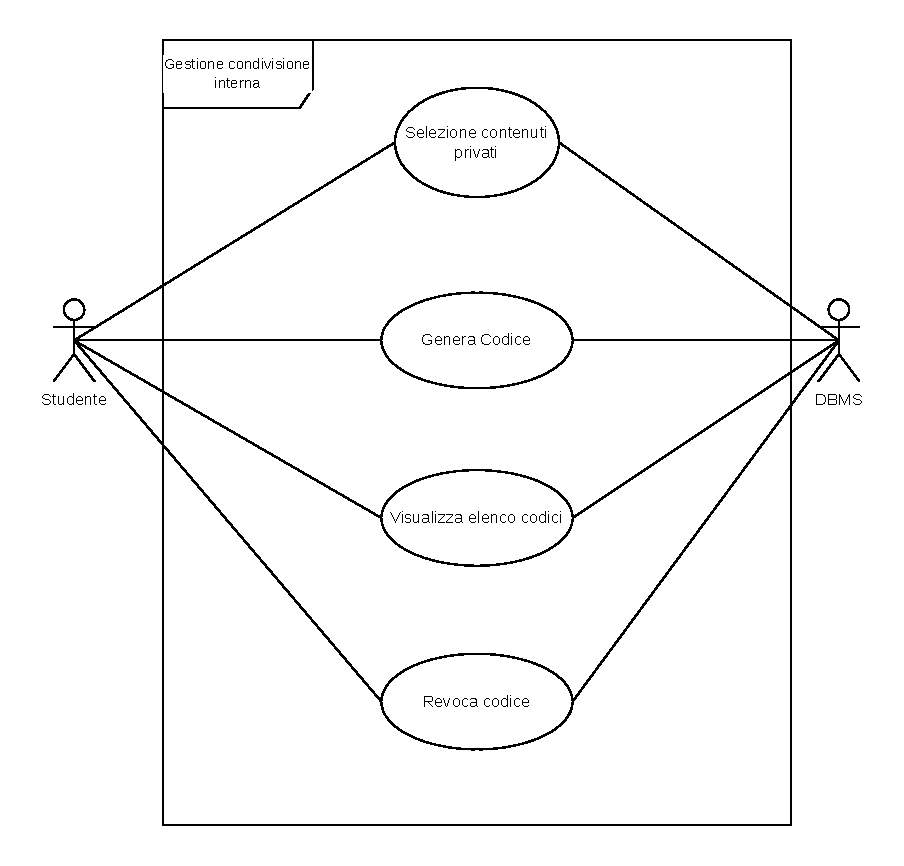
\includegraphics[width=\textwidth,height=1.2\textheight,keepaspectratio]{pdf/GestioneCondivisioneInterna/VistaD'insiemeProgetto-2-Gest cond interna.drawio.pdf}
    \caption{Vista d'insieme di Gestione Condivisione Interna}
    \label{fig:gest_condInt}
\end{figure}

\newpage

\subparagraph{Selezione Contenuti Privati}

\footnotesize
\begin{longtable}{|
>{\columncolor{unipablue}\color{white}\bfseries\raggedright\arraybackslash}p{3.4cm}|
>{\raggedright\arraybackslash}p{10.2cm}|}
\hline
Caso d'uso & Selezione Contenuti Privati \\ \hline
ID & 7.1 \\ \hline
Attori & Studente, DBMS \\ \hline
Precondizioni & Il Sistema ha mostrato a video la schermata ``Home AFAM''. \\ \hline
Flusso degli eventi &
\begin{enumerate}[topsep=0.2em,itemsep=0.15em,parsep=0pt,partopsep=0pt]
    \item Lo studente clicca sulla sezione ``Gestione Condivisione Interna''.
    \item Il Sistema mostra a video la schermata ``Gestione Condivisione Interna''.
    \item Lo studente clicca sul pulsante ``Seleziona Contenuti Privati''.
    \item Il Sistema recupera dalla memoria temporanea i dati dello studente.
    \item Il Sistema interroga il DBMS per recuperare i file privati.
    \item \textbf{SE} lo studente non ha alcun contenuto caricato:
    \begin{itemize}[topsep=0.15em,itemsep=0.1em,parsep=0pt,partopsep=0pt]
        \item[6.1.] Il Sistema mostra a video il messaggio di errore: ``Nessun contenuto disponibile''.
        \item[6.2.] Lo studente clicca sul pulsante ``OK'' per chiuderlo.
        \item[6.3.] Il Sistema mostra nuovamente la schermata ``Gestione Condivisione Interna''.
    \end{itemize}
    \item \textbf{ALTRIMENTI} (ci sono contenuti disponibili):
    \begin{itemize}[topsep=0.15em,itemsep=0.1em,parsep=0pt,partopsep=0pt]
        \item[7.1.] Il Sistema mostra a video la schermata ``Seleziona Contenuti Privati'', contenente l'elenco dei file e il pulsante ``Conferma Selezione Finale''.
        \item[7.2.] Lo studente seleziona i contenuti che desidera condividere.
        \item[7.3.] Lo studente clicca sul pulsante ``Conferma Selezione Finale''.
        \item[7.4.] Il Sistema mostra a video la schermata ``Generazione Codice''.
    \end{itemize}
\end{enumerate} \\ \hline
Postcondizioni &
\begin{enumerate}[topsep=0.2em,itemsep=0.15em,parsep=0pt,partopsep=0pt]
    \item Il Sistema ha mostrato a video la schermata ``Generazione Codice''.
    \item Il Sistema ha mostrato la schermata ``Gestione Condivisione Interna''.
\end{enumerate} \\ \hline
\caption{Scheda di dettaglio del Caso d'Uso Selezione Contenuti Privati}
\label{tab:uc_selezione_contenuti_privati}\\
\end{longtable}
\normalsize

\newpage
\subparagraph{Genera Codice}

\small
\begin{longtable}{|
>{\columncolor{unipablue}\color{white}\bfseries\raggedright\arraybackslash}p{3.4cm}|
>{\raggedright\arraybackslash}p{10.2cm}|}
\hline
Caso d'uso & Genera Codice \\ \hline
ID & 7.2 \\ \hline
Attori & Studente, DBMS \\ \hline
Precondizioni & Il Sistema ha mostrato a video la schermata ``Generazione Codice''. \\ \hline
Flusso degli eventi &
\begin{enumerate}[topsep=0.2em,itemsep=0.15em,parsep=0pt,partopsep=0pt]
    \item Lo studente clicca sul pulsante ``Genera Codice''.
    \item Il Sistema genera un codice univoco associato ai file selezionati.
    \item Il Sistema invia i dati del codice generato, l'elenco dei file associati e l'identificativo dello studente al DBMS per la memorizzazione definitiva.
    \item Il Sistema mostra a video un messaggio di conferma: ``Codice generato con successo'', contenente il codice testuale creato e i pulsanti ``Copia Codice'' e ``OK''.
    \item Lo studente clicca sul pulsante ``Copia Codice''.
    \item Il Sistema copia il codice generato nel dispositivo dello studente.
    \item Lo studente clicca sul pulsante ``OK'' per chiudere il messaggio di conferma.
    \item Il Sistema mostra a video la schermata ``Gestione Condivisione Interna''.
\end{enumerate} \\ \hline
Postcondizioni & Il Sistema ha mostrato a video la schermata ``Gestione Condivisione Interna''. \\ \hline
\caption{Scheda di dettaglio del Caso d'Uso Genera Codice}
\label{tab:uc_genera_codice}\\
\end{longtable}
\normalsize

\newpage
\subparagraph{Visualizza Elenco Codici}

\footnotesize
\begin{longtable}{|
>{\columncolor{unipablue}\color{white}\bfseries\raggedright\arraybackslash}p{3.4cm}|
>{\raggedright\arraybackslash}p{10.2cm}|}
\hline
Caso d'uso & Visualizza Elenco Codici \\ \hline
ID & 7.3 \\ \hline
Attori & Studente, DBMS \\ \hline
Precondizioni & Il Sistema ha mostrato a video la schermata ``Gestione Condivisione Interna''. \\ \hline
Flusso degli eventi &
\begin{enumerate}[topsep=0.2em,itemsep=0.15em,parsep=0pt,partopsep=0pt]
    \item Lo studente clicca sulla sezione ``Gestisci Codici''.
    \item Il Sistema recupera dalla memoria temporanea l'identificativo dello studente.
    \item Il Sistema interroga il DBMS per recuperare la lista dei codici generati dallo studente.
    \item \textbf{SE} lo studente non possiede alcun codice generato:
    \begin{itemize}[topsep=0.15em,itemsep=0.1em,parsep=0pt,partopsep=0pt]
        \item[4.1.] Il Sistema mostra a video il messaggio di errore: ``Nessun codice generato''.
        \item[4.2.] Lo studente clicca sul pulsante ``OK''.
        \item[4.3.] Il Sistema mostra a video la schermata ``Gestione Condivisione Interna''.
    \end{itemize}
    \item \textbf{ALTRIMENTI} (ci sono codici generati):
    \begin{itemize}[topsep=0.15em,itemsep=0.1em,parsep=0pt,partopsep=0pt]
        \item[5.1.] Il Sistema mostra a video la schermata ``Elenco Codici'', contenente l'elenco dei codici e il pulsante ``Revoca''.
    \end{itemize}
\end{enumerate} \\ \hline
Postcondizioni &
\begin{enumerate}[topsep=0.2em,itemsep=0.15em,parsep=0pt,partopsep=0pt]
    \item Il Sistema ha mostrato a schermo la schermata ``Elenco Codici''.
    \item Il Sistema ha mostrato a video la schermata ``Gestione Condivisione Interna''.
\end{enumerate} \\ \hline
\caption{Scheda di dettaglio del Caso d'Uso Visualizza Elenco Codici}
\label{tab:uc_visualizza_elenco_codici}\\
\end{longtable}
\normalsize

\newpage
\subparagraph{Revoca Codice}

\small
\begin{longtable}{|
>{\columncolor{unipablue}\color{white}\bfseries\raggedright\arraybackslash}p{3.4cm}|
>{\raggedright\arraybackslash}p{10.2cm}|}
\hline
Caso d'uso & Revoca Codice \\ \hline
ID & 7.4 \\ \hline
Attori & Studente, DBMS \\ \hline
Precondizioni & Il Sistema ha mostrato a video la schermata ``Elenco Codici''. \\ \hline
Flusso degli eventi &
\begin{enumerate}[topsep=0.2em,itemsep=0.15em,parsep=0pt,partopsep=0pt]
    \item Lo studente clicca sul pulsante ``Revoca'' in corrispondenza di un codice specifico.
    \item Il Sistema mostra a video un messaggio di conferma: ``Sei sicuro di voler revocare questo codice?'', con il pulsante ``Conferma''.
    \item Lo studente clicca sul pulsante ``Conferma''.
    \item Il Sistema invia la richiesta di revoca al DBMS per aggiornare lo stato del codice.
    \item Il Sistema mostra nuovamente la schermata ``Elenco Codici''.
\end{enumerate} \\ \hline
Postcondizioni & Il Sistema ha mostrato a schermo la schermata ``Elenco Codici''. \\ \hline
\caption{Scheda di dettaglio del Caso d'Uso Revoca Codice}
\label{tab:uc_revoca_codice}\\
\end{longtable}
\normalsize



\end{document}
